\chapter{Aesthetic ideals in programming practices}
\label{chap:ideals}

The first step in our study of aesthetic standards in source code will identify the aesthetic ideals ascribed by programmers to the source code they write and read; that is, the syntactic qualifiers and semantic fields that they refer to when discussing program texts. To that end, we first start by clarifying whom we refer to by the term \emph{programmers}, revealing a multiplicity of practices and purposes, from massively-distributed codebases to \emph{ad hoc}, one-line solutions, cryptic puzzles and printed code.

We then turn to the kinds of beauty that these programmers aspire to. After expliciting our methodology of discourse analysis, we engage in a review of the various kinds of publications that make up programmers' discourses, in which they qualify their practice. Out of these, we identify a cluster of adjectives and comparisons which will provide an empirical basis for considering the desirable and undesirable aesthetic properties of source code.

We then move to a description of which aesthetic fields are being referenced by programmers on a broader level, and consider how multiple kinds of beauties, from literary, to scientific and architectural conceptions of beauty can overlap and be referred to in the same medium. Such an overlap will reveal the importance of function, craft and knowledge in the disposition and representation of code. Our conclusion focuses on how understanding plays a central role in an aesthetic approach to source code, and results from the specificity of code as a cognitive material.

\section{The practices of programmers}
\label{sec:practice-programmers}

The history of software development is that of a practice born in the aftermath of the second world war, one which trickled down to broader and broader audiences at the eve of the twenty-first century. Through this development, various paradigms, platforms and applications have been involved in producing software, resulting in different epistemic communities \citep{cohendet_organisational_2001} and communities of practice \citep{hayes_cultures_2017}, in turn producing different types of source code. Each of these write source code with particular characteristics, and with different priorities in how knowledge is produced, stored, exchanged, transmitted and retrieved. In this section, we take a socio-historical stance on the field of programming, highlighting how diverse practices emerge at different moments in time, how they are connected to contemporary technical and economic organizations, and for specific purposes. Even though such types of reading and writing source code often overlap with one another, this section will highlight a diversity of  ways in which code is written, notably in terms of origin—how did such a practice emerge?—, references—what do they consider good?—, purposes—what do they write for?—and examples—how does their code look like?.

First, we take a look at the software industry, to identify professional \emph{software developers}, the large program texts they work on and the specific organizational practices within which they write it. They are responsible for the majority of source code written today, and do so in a professional and productive context, where maintainability, testability and reliability are the main concerns. Then, we turn to a parallel practice, one that is often exhibited by software developers, as they also take on the stance of \emph{hackers}. Disambiguating the term reveals a set of practices where curiosity, cleverness, and idiosyncracy are central, finding unexpected solutions to complex problems, sometimes within artificial and playful constraints. \emph{Scientists} operate within an academic environment, focusing on concepts such as simplicity, minimalism and elegance; they are often focused on theoretical issues, such as mathematical models, as well as programming language design, but are also involved in the implementation of algorithms. Finally, \emph{poets} read and write code first and foremost for its textual and semantic qualities, publishing code poems online and in print, and engaging deeply with the range of metaphors allowed by this dynamic linguistic medium.

While this overview encompasses most of the programming practices, we leave aside some approaches to code, mainly because they do not directly engage with the representation of source code as a textual matter. More and more, end-user applications provide the possibility to program in rudimentary ways, something referred to as the "low-code" approach \citep{team_lowcode_2021}, and thus contributing to the blurring of boundaries between programmers and non-programmers\footnote{For instance, Microsoft's Visual Basic for Applications, Ableton's Max For Live, MIT's Scratch or McNeel's Grasshopper are all programming frameworks which are not covered within the scope of this study. In the case of VBA and similar office-based high-level programming, it is because such a practice is a highly personal and \emph{ad hoc} one, and therefore is less available for study.}.

\subsection{Software developers}
\label{subsec:software-developers}

As Niklaus Wirth puts it, \emph{the history of software is the history of growth in complexity} \citep{wirth_brief_2008}, while also following a constant lowering of the barrier to entry to the tools through which this complexity is managed. As computers' technical abilities in memory storage and processing power increased year on year since the 1950s, the nature of writing computer instructions shifted as well.

\subsubsection{From machine dependence to autonomous language}
\label{subsubsec:from-machine-to-language}

In his history of the software industry, Martin Campbell-Kelly traces the development of a discipline through an economic and a technological lens, and he identifies three consecutive waves in the production of software \citep{campbell-kelly_airline_2003}. Starting in the 1950s, and continuing throughout the 1960s, software developers were contractors hired to work directly with a specific hardware. These mainframes were large, expensive, and rigid machines, requiring platform-specific knowledge of the corresponding Assembly instruction set, the only programming language available at the time\footnote{One of the first operating systems, MIT's Tape Director, would be only developped in 1956 \citep{ross_personal_1986}, which would facilitate some of the more basic memory allocation, process management, and system calls}. Two distinct groups of people were involved in the operationalization of such machine: electrical engineers, tasked with designing hardware, and programmers, tasked with implementing the software. While the former historically received the most attention \citep{ross_personal_1986}, the latter was mostly composed of women and, as such, not considered essential in the process \citep{light_when_1999}. At this point, then, programming remains hardware-dependent\footnote{\emph{But most important of all, the programmer himself had a very modest view of his own work: his work derived all its significance from the existence of that wonderful machine. Because that was a unique machine, he knew only too well that his programs had only local significance and also, because it was patently obvious that this machine would have a limited lifetime, he knew that very little of his work would have a lasting value. Finally, there is yet another circumstance that had a profound influence on the programmer's attitude to his work: on the one hand, besides being unreliable, his machine was usually too slow and its memory was usually too small, i.e. he was faced with a pinching shoe, while on the other hand its usually somewhat queer order code would cater for the most unexpected constructions. And in those days many a clever programmer derived an immense intellectual satisfaction from the cunning tricks by means of which he contrived to squeeze the impossible into the constraints of his equipment.} \citep{dijkstra_humble_2007}}.

In the 1960s, hardware switched from vacuum tubes to transistors and from magnetic core memory to semiconductor memory, making them faster and more capable to handle complex operations.  On the software side, the development of several programming languages, such as FORTRAN, LISP and COBOL, started to address the double issue of portability—having a program run unmodified on different machines—and expressivity—expressing a program text in a high-level, English-like syntax, rather than Assembly instruction codes. Programmers are no longer tied to a specific machine, and therefore acquire a certain autonomy, a recognition which culminates in the naming of the field of \emph{software engineering} \citep{randell_nato_1996}.

Campbell-Kelly concludes on a wave of mass-market production: following the advent of the UNIX family of operating systems, the distribution of the C programming language, the wide availability of C compilers, and the appearance of personal computers such as the Commodore 64, Altair and Apple II, software could be effectively entirely decoupled from hardware. The writing of software is no longer a corollary to the design of hardware, and as an independent field would as such become the main focus of computing as a whole \citep{ceruzzi_history_2003}. And yet, software immediately enters a crisis, where projects run over time and budget, prove to be unreliable in production and unmaintainable in the long-run. It is at this time that discussions around best practices in writing source code started to emerge.

This need for a more formal approach to the actual process of programming found one of its most important manifestations in Edsger Dijkstra's \emph{Notes on Structured Programming} \citep{dijkstra_chapter_1972}. In it, he argues for moving away from programming as a craft, and towards programming as an organized discipline, with its methodologies and systematization of program construction. Despite its laconic section titles\footnote{See, for instance, Chapter 1: "\emph{On our inability to do much}"}, Dijkstra's 1972 report nonetheless contributed to establish a more rigorous typology of the constructs required for reliable, provable programs—based on fundamental heuristics such as sequencing, selection, iteration and recursion—, and aimed at the formalization of the practice. Along with other subsequent developments (such as Hoare's contribution on proper data structuring \citep{hoare_chapter_1972}, or the rise of object-oriented programming with Smalltalk \citep{kay_early_1993}) programming would solidify its foundations as a profession:

\begin{quote}
  We knew how the nonprofessional programmer could write in an afternoon a three-page program that was supposed to satisfy his needs, but how would the professional programmer design a thirty-page program in such a way that he could really justify his design? What intellectual discipline would be needed? What properties could such a professional programmer demand with justification from his programming language, from the formal tool he had to work with?  \citep{dijkstra_chapter_1972}
\end{quote}

As a result of such interrogations comes an industry-wide search for solutions to the intractable problem of programming: that it is \emph{a technique to manage information which in turn produces information}. To address such a conundrum, a variety of tools, formal methods and management processes enter the market; they aim at acting as a \emph{silver bullet} \citep{brooksjr_mythical_1975}, a magical solution addressing the cascade of potential risks which emerge from large software applications\footnote{For instance, the \emph{Forum on Risks to the Public in Computers and Related Systems} serves as a publication to centralize such concerns \citep{neumann_computerrelated_1985}}. This growth in complexity is also accompanied by a diversification of software applications: as computers become more widely available, and as higher-level programming languages provide more flexibility in their expressive abilities, software engineering engages with a variety of domains, each of which might need a specific solution, rather than a generic process. Confronted with this diversity of applications, business literature on software practices flourishes, being based on the assumption that the complexity of software should be tackled at its bottleneck: the reading and writing of source code.

The most recent wave in the history of software developers is the popularization of the Internet and of the World Wide Web, a network which was only standardized in 1982 and access to it was provided commercially in 1989. Built on top of the Internet, it popularized global information exchange, including technical resources to read and write code. Software could now be written on cloud computing platforms, shared through public repositories and deployed via containers with a lower barrier to entry than at a time of source code printed in magazines, of overnight batch processing and of non-time-sharing systems.

\subsubsection{Engineering texts}
\label{subsubsec:engineering-texts}

Software developers have written some of the largest program texts to this date. However, due to its close ties to commercial distributors, source code written in this context often falls under the umbrella of proprietary software, thus made unavailable to the public. The program texts written by software developers are large, they often feature multiple programming languages and are highly structured and standardized: each file follows a pre-established convention in programming style, which supports an authoring by multiple programmers without any obvious trace to a single individual authorship. These program texts stand the closest to a programming equivalent of engineering, with its formalisms, standards, usability and attention to function.

The IEEE's Software Engineering Body of Knoweldge (SWEBOK) provides a good starting point to survey the specificities of software developers as source code writers and readers \citep{bourque_swebok_2014}; the main features of which include the definition of requirements, design, construction, testing and maintenance. Software requirements are the acknowledgement of the importance of the \emph{problem domain}, the domain to which the software takes its inputs from, and to which it applies its outputs. For instance, software written for a calculator has arithmetic as its problem domain; software written for a learning management system has students, faculty, education and courses as its problem domain; software written a banking institution has financial transactions, savings accounts, fraud prevention and credit lines as its problem domain. This essential step in software development aims at formalizing as best as possible the elements that exist beyond software, in order to make those computable, and the design of an adequate formalism is a fundamental requirement for a successful software application.

Software design relates to the overall organization of the software components, considered not in their textual implementation, but in their conceptual agency. Usually represented through diagrams or modelling languages, it is concerned with \emph{understanding how a system should be organized and designing the overall structure of that system} \citep{sommerville_software_2010}. Of particular interest is the relationship that is established between software development and software architecture. Software architecture operates both from a top-down perspective, laying down an abstract blueprint for the implementation of a system and dictating how a program text is structured, how its parts interact, why it's built that way, consisting different components of an existing system interact \citep{brown_architecture_2011}.

Software construction relates to the actual writing of software, and how to do so in the most reliable way possible. The SWEBOK emphasizes first and foremost the need to minimize complexity\footnote{Complexity does not exist only at the programming level, but also at the architecture level: \emph{"there are two ways of constructing a software design: one way is to make it so simple that there are obviously no deficiencies, and the other way is to make it so complicated that there are no obvious deficiencies."} \citep{hoare_emperor_1981}}, in anticipation of likely changes and possible reuse by other software systems. Here, the emphasis on engineering is particularly salient: while most would refer to the creation of software as \emph{writing} software, the IEEE document refers to it as \emph{constructing} software: the creation of working software through a combination of coding, verification, unit testing, integration testing, and debugging. \citep{bourque_swebok_2014}. The practice of software engineers thus implements functional and reliable mechanical designs through, ultimately, the act of writing in formal languages.

Software maintenance, finally, relates not to the planning or writing of software, but to its reading. Software is notoriously filled with bugs\footnote{McConnell estimates that the industry average is about 15 - 50 errors per 1000 lines of delivered code. \citep{mcconnell_code_2004}.} which can be fixed through the release of software updates. This means that the life of a software doesn't stop when its first version is written, but rather when it does not run anywhere anymore: it can still be edited across time and space, by other programmers which might not have access to the original group of implementers: consequently, software should be first and foremost understandable—SWEBOK lists the first feature of coding as being \emph{techniques for creating understandable source code} \citep{bourque_swebok_2014}. This final component of software development directs us back to its notorious cognitive complexity, one that increases with the age of the software.

What does this look like in practice? In order to understand the aesthetic preferences of software developers, we must start by assessing the kinds of program texts they write. We look at excerpts from two code bases: the source code for Microsoft Windows XP, which was started in 2001 \citep{warren_windows_2020}, and the Kirby CMS project, started in 2011; the quantitative specificities of both code bases are shown in \ref{table:ms-kirby}. While these two projects differ drastically in their size, in their age, and in the number of developers involved in their creation and maintenance, we nonetheless choose them as the respective ends of a single spectrum of software engineering. In both cases, the prime concern is with function and maintainability.

\begin{table}
  \begin{tabular}{lll}
                              & Microsoft XP & Kirby CMS \\
    \hline
    number of files           & 28,655       & 1,859     \\
    \hline
    total lines               & 13,468,327   & 345,793   \\
    \hline
    number of file extensions & 10           & 6
  \end{tabular}
  \caption{Table comparing the scale of two software development projects.}
  \label{table:ms-kirby}
\end{table}

First, the most striking visual feature of the code is its sheer size. In the case of Microsoft XP, representing such a versatile and low-level application such as an operating system results in files that are often above 2000 lines of code. In order to allow abstraction techniques at a higher-level for the end-developer, the operating system needs to do a significant amount of "grunt" work, relating directly to the concrete reality of the hardware platform which needs to be operated on. Looking at the file \lstinline{cmdatini.c}, reproduced partially in \ref{code:ms2000}, we see very long variable names, with a rhythmic, repetitive structure where differences between lines is not obivous at first.

\begin{listing}
  \inputminted{c}{./corpus/ms2000_abridged.c}
  \caption{Unicode string initialization in Microsoft 2000 operating system, with a first part showing an explicit repeating pattern, while the second part shows a more compressed approach.}
  \label{code:ms2000}
\end{listing}

The repetition of the \lstinline{RtlInitUnicodeString} in the first part of this listing stands at odds with the second part of the code, the \lstinline{for()} statement, displaying a contrast between between a verbose text and a compressed text. Verbosity, the act of explicitly writing out statements which could be functionally equivalent in a compacted form, is a feature of the Windows 2000 codebase, one which is a consequence of a particular problem domain, of a particular business imperative of maintainability, and of the particular semantic environment of the C programming language.

The problem domain of the Windows XP operating system, its longevity and its update cycle, all contribute to its complexity and have affected how this code is written. Here, the problem domain of the program text is the computer hardware, and its function is to make sure the kernel knows about the hardware it is running on (e.g. its name, its description, etc.), in an explicit and verbose way, before more compressed writing techniques can be used. Dealing with a specific problem domain (i.e. kernel instructions) leads to a specific kind of aesthetics; here, forcing the programmers to repeat references to \lstinline{RtlInitUnicodeString()} 1580 times across 336 files.

Another significant aesthetic feature of the Windows 2000 program text is its use of comments, and how those comments point to a collaborative, layered authorship. This particular program text is written across individuals and across time, each with presumably its own approach. Yet, writing source code within a formal organization often implies the harmonization of individual approaches, and thus the adoption of coding styles, with the intent that \emph{all code in any code-base should look like a single person typed it, no matter how many people contributed} \citep{waldron_idiomatic_2020}. The excerpt in \ref{code:buffer_c} from \lstinline{jdhuff.c} is a example of such overlapping of styles.

\begin{listing}
  \inputminted[]{c}{./corpus/buffer.c}
  \caption{Overlapping programming voices can be hinted at by different comment styles.}
  \label{code:buffer_c}
\end{listing}

Comments are specific lines of source code, identified by particular characters (in the C programming language, they are marked using \lstinline{//} and \lstinline{/* */}), which are ignored by the machine. That is, they are only expected to be read by other programmers, and in this case primarily by programmers belonging to a single business organization. Here, the variety of comment characters and the variety of capitalization hint at the various origins of the authors, or at the very least at the different moments, and possible mental states of the potential single-author.

Treated as natural language, comments are not procedurally guaranteed to be reflected in the execution, of the program, and are considered by some as misleading: they might be saying something, while the code does something else\footnote{This has led to the argument that only the source code has epistemological value in a software project: "\emph{the only document that describes your code completely and correctly is the code itself}" \citep{goodliffe_code_2007}}. Beyond the presence of multiple authors, this excerpt also exemplifies the tension between source code as the canonical source of knowledge of what the program does and how it does it and comments as a more idiosyncratic dimension of all natural-language expressions of human programmers.

And yet, this chronological and interpersonal spread of the program text, combined with organizational practices, require the use of comments in order to maintain aesthetic and cognitive coherence in the program. This is the case in the use of comment headers, which locate a specific file within the greater architectural organization of the program text (see \ref{code:enum_c}). This highlights the multiple authors and the evolution in time of the file: comments are the only manifestation of this layering of revisions which ultimately results in the "final" software\footnote{The term "final" is in quotes, since the Windows 2000 source contains the mention \lstinline{BUGBUG} 7436 times across 2263 files, a testament to the constant state of unfinishedness that software tends to remain in.}.

\begin{listing}
  \inputminted{c}{./corpus/enum.c}
  \caption{pnpenum.c shows the explicit traces of multiple authors collaborating on a single file over time.}
  \label{code:enum_c}
\end{listing}

Ultimately, the Windows XP source code shows some of the components at stake in the program texts written by software developers: verbosity and compression, multi-auctoriality, and natural language writing in the midst of formal languages. Still, as an operating system developed by one of the largest corporations in the world, it also possesses some specificities due to its problem domain, programming language and socio-economic environment.

Another example of a program text written by software developers, complementing Windows XP, is the Kirby CMS \citep{allgeier_kirby_2022}. With development starting in 2011 and a first release in 2012, it developed a steady community of susers, shown in consistent forum posts and commit history on the main repository. Kirby is open-source, meaning that it affords direct engagement of other developers with its architecture through modification, extension or partial replacement, content management system. Its problem domain is therefore the organization of user-facing multimedia assets, such as text, images and videos.

The Kirby source code is entirely available online, and the following snippets hint at another set of formal values—conciseness, expliciteness and delimitation. Conciseness can be seen in the lengths of the various components of the code base. For instance, the core of Kirby consists in 1859 files, with the longest being \lstinline{src/Database/Query.php} at 1065 lines, and the shortest being \lstinline{src/Http/Exceptions/NextRouteException.php} at 16 lines, for an average of 250 lines per file \footnote{As a comparison, the leading project in the field, Wordpress.org, has 3466 files, with the longest file comprising 9353 lines of code (\lstinline{customize-controls.js}), and the shortest 1line (such as \lstinline{script-loader-packages.php}) \citep{wordpress_wordpress_2023}}.

If we look at a typical function declaration within Kirby, we found one such as the \lstinline{distinct()} setter for Kirby's database, reproduced in \ref{code:query_php}. This function allows the developer to set whether she only wants to select distinct fields in a database query.

\begin{listing}
  \inputminted{php}{./corpus/query.php}
  \caption{The setting of whether a query should be distinct includes some verbose details which prove to be helpful in the long run \citep{allgeier_query_2021}.}
  \label{code:query_php}
\end{listing}

Out of these 11 lines, the actual functionality of the function is focused on one line, \lstinline{$this->distinct = $distinct;}. Around it are machine-readable comment snippets, and a function wrapper around the simple variable setting. The textual overhead then comes from the wrapping itself: the actual semantic task of deciding whether a query should be able to include distinct select clauses (as opposed to only allowing join clauses), is now decoupled from its actual implementation. The quality of this writing, at first verbose, actually lies in its conciseness in relation to the possibilities for extension that such a form of writing allows: the \lstinline{distinct()} function could, under other circumstances, be implemented differently, and still behave similarly from the perspective of the rest of the program. Additionally, this wrapping enables the setting of default values (here, \lstinline{true}), a minimal way to catch bugs by always providing a fallback case.

Kirby's source code is also interestingly explicit in comments, and succint in code. Taking from the \lstinline{Http\\Route} class, reproduced in \ref{code:route_php}, we can see a different approach to comments than in \ref{code:buffer_c} of Microsoft XP operating system.

\begin{listing}
  \inputminted{php}{./corpus/route.php}
  \caption{The inclusion of comments help guide a programmer through an open-source project \citep{allgeier_route_2021}.}
  \label{code:route_php}
\end{listing}

The 9 lines above the function declaration are machine-readable documentation. It can be parsed by a programmatic system and used as input to generate more classical, human-readable documentation in the form of a website or a printed document. This is noticeable due to the highly formalized syntax \lstinline{param string name_of_var}, rather than writing out "this function takes a parameter of type string named \lstinline{name_of_var}". This does compensate for the tendency of comments to drift out of synchronicity with the code that they are supposed to comment, by tying them back to some computational system to verify its semantic contents, while providing information about the inputs and outputs of the function. Once again, we see that the source of truth is the computer's ability of reading input and executing it.

Beyond expliciting inputs and outputs, the second aspect of these comments is targeted at the \emph{how} of the function, helping the reader understand the rationale behind the programmatic process. Comments here aren't cautionary notes on specific edge-cases, as seen in \ref{code:route_php}, or on generic meta-information, but rather natural language renderings of the thought process of the programmer. The implication here is to provide a broader, and more explicit understanding of the process of the function, in order to allow for further maintenance, extension or modification.

Finally, we look at a subset of the function, the clause of the third if-statement: \lstinline{(preg_match('#^' . $this->regex($pattern) . '$#u', $path, $parameters))}. Without comments, one must realize on cognitive gymnastics and knowledge of the PHP syntax in order to render this as an extraction of all route parameters, implying the removal of the first element of the array. In this sense, then, Kirby's code for parsing an HTTP route is both verbose in comments and parsimonious in code. The reason for those comments becomes clear: that the small core of the function is actually hard to understand.

Looking at some excerpts from the Kirby program texts, we see a small number of files, overall short file length, short function length, consistent natural language comments and concise functionality. These aesthetic features give an impression of building blocks: short, graspable, (re-)usable components are made available to the developer directly, as the open-source project relies on contributions from individuals who are not expected to have any other encounter with the project other than, at the bare minimum, the source code itself.

\begin{listing}
  \inputminted{js}{./corpus/clipboard.js}
  \caption{Even in a productive and efficient open-source project, one can detect traces of "hacks" \citep{allgeier_clipboard_2021}.}
  \label{code:clipboard_js}
\end{listing}

In conclusion, these two examples of program texts written by software developers, Microsoft Windows XP and Kirby CMS, show particular presentations of source code—such as repetition, verbosity, commenting and conciseness. These are in part tied to their socio-technical ecosystems made up of hardware, institutional practices ranging from corporate guidelines to open-source contribution, with efficiency and usability remaining at the forefront, at least in its executed form.

Indeed, software developers are a large group of practitioners whose focus is on producing effective, reliable and sustainable software. This leads them to writing in a relatively codified manner. And yet, we must acknowledge that idiosyncracies in source code emerge; in \ref{code:clipboard_js}, a function handling text input uses a convoluted workaround to store text data. Even in business environments and functional tools, then, the hack is never too far. The boundary between groups of practitioners is not clear-cut, and so we now turn to the correlated practice of hackers.

\subsection{Hackers}
\label{subsec:hackers}

To hack, in the broadest sense, is to enthusiastically inquire about the possibilities of exploitation of technical systems\footnote{"HACKER [originally, someone who makes furniture with an axe] n. 1. A person who enjoys learning the details of programming systems and how to stretch their capabilities, as opposed to most users who prefer to learn only the minimum necessary. 2. One who programs enthusiastically, or who enjoys programming rather than just theorizing about programming. \citep{dourish_original_1988}}. Computer hacking specifically came to proeminence as early computers started to become available in north-american universities, and coalesced around the Massachussets Institute of Technology's Tech Model Railroad Club \citep{levy_hackers_2010}. Computer hackers were at the time skilled and highly-passionate individuals, with an autotelic inclination to computer systems: these systems mattered most when they referenced themselves, instead of interfacing with a given problem domain. Early hackers were often self-taught, learning to tinker with computers while still in high-school \citep{lammers_programmers_1986}, and as such tend to exhibit a radical position towards expertise: skill and knowledge aren't derived from academic degrees or credentials, but rather from concrete ability and practical efficacy\footnote{A meritocratic stance which has been analyzed in further in  \citep{coleman_aesthetics_2018}}.

The histories of hacking and of software development are deeply intertwined: some of the early hackers worked on software engineering projects—such as the graduate students who wrote the Apollo Guidance Computer routines under Margaret Hamilton—and then went on to profoundly shape computer infrastructure. Particularly, the development of the UNIX operating system by Dennis Ritchie and Ken Thompson is a key link in connecting hacker practices and professional ones. Developed from 1969 at Bell Labs, AT\&T's research division, UNIX was a product at the intersection of corporate and hacker culture, built by a small team, circulating along more or less legal channels, and spreading its design philosophy of clear, modular, simple and transparent design across programming communities \citep{raymond_art_2003}.

Hacker culture built on this impetus to share source code, and hence to make written software understandable from its textual manifestation. As hardware stopped being the most important component of a computing system to software had led manufacturers to stop distributing source code, making proprietary software the norm. Until then, executable software was the consequence of running the source code through a compilation process; around the 1980s, executable software was distributed directly as a binary file, its exact contents an unreadable series of 0s and 1s.

In the meantime, personal microcomputers came to the market and opened up this ability to tinker and explore computer systems beyond the realms of academic-licensed large mainframes and operating systems. Starting with models such as the Altair 8800, the Apple II and the Commodore 64, as well as with easier, interpreted computer languages such as BASIC, whose first version for such micro-computers was written by Bill Gates, Paul Allen and Monte Davidoff \citep{montfort_10_2014}. While seemingly falling out of the realm of "proper" programming, the microcomputer revolution allowed for new groups of individuals to explore the interactivity of source code due to their small size when published as type-in listings.

In the wake of the larger free software movement, emerged its less radical counterpart, the open-source movement, as well as its more illegal counterpart, security hacking. The latter is usually represented by the types of individuals depicted in mainstream news outlets when they reference hackers: programmers breaching private systems, sometimes in order to cause financial, intelligence or material harm. Security hackers, sometimes called crackers, form a community of practice of their own, with ideas of superior intelligence, subversion, adventure and stealth\footnote{For a lyrical account of this perception of the hacker ethos, see \emph{The Conscience of a Hacker}, published in Phrack Magazine: "This is our world now\dots{} the world of the electron and the switch, the beauty of the baud.  We make use of a service already existing without paying for what could be dirt-cheap if it wasn't run by profiteering gluttons, and you call us criminals.  We explore\dots{} and you call us criminals.  We seek after knowledge\dots{} and you call us criminals." \citep{mentor+++_conscience_1986}}. These practices nonetheless refer to the original conception of hacking—getting something done quickly, and well—and include such a practical, efficient appoach into its own set of values and ideals. In turn, these are represented in the kinds of program texts being written by members of this community of practice.

Meanwhile, the open-source movement took the tenets of hacking culture and adapted it to make it more compatible to the requirements of businesses. Indeed, beyond the broad values of intellectual curiosity and skillful exploration, free software projects such as the Linux kernel, the Apache server or the OpenSSL project have proven to be highly efficient, and used in both commercial, non-commercial, critical and non-critical environments \citep{raymond_cathedral_2001}. Such an approach sidesteps the political and ethical values held in previous iterations of the hacker ethos in order to focus exclusively on the sharing of source code and open collaboration while remaining within an inquisitive and productive mindframe. With the advent of corporate \emph{hackathons}—short instances of intense collaboration in order to create new software, or new features on a software system—are a particularly salient example of this overlap between industry practices and hacker practices \citep{nolte_you_2018}\footnote{Another overlap can be found in the address of the software corporate giant Meta's headquarters: 1, Hacker Way, Menlo Park, CA 94025, U.S.A.}.

As a community of practice, hackers are programmers which, while overlapping with industry-embedded software developers, hold a set of values and ideals regarding the purpose and state of software. Whether academic hackers, amateurs, security hackers or open-source contributors, all are centered around the object of source code as a vehicle for communicating the knowledge held within the software, the necessity of skill for writing such software, and a certain inclination towards "quick and dirty" solutions.

\subsubsection{Program texts as puzzles}
\label{subsubsec:program-texts-puzzles}

Incidentally, those political and ethical values of expertise and openness often overlap with aesthetic values informing how their code exists in its textual manifestation. By looking at a few program texts written by hackers, we will see how their skillful engagment with the machine, and their playful stances towards solving problems is also reflected in how they write source code.

\begin{quote}
  To hack is, according to the dictionary, "to cut irregularly, without skill or definite purpose; to mangle by or as if by repeated strokes of a cutting instrument". I have already said that the compulsive programmer, or hacker as he calls himself, is usually a superb technician. It seems therefore that he is not "without skill" as the definition will have it. But the definition fits in the deeper sense that the hacker is "without definite purpose": he cannot set before him a clearly defined long-term goal and a plan for achieving it, for he has only technique, not knowledge. He has nothing he can analyze or synthesize; in short, he has nothing to form theories about. His skill is therefore aimless, even disembodied. It is simply not connected with anything other than the instrument on which it may be exercised. His skill is that of a monastic copyist who, though illiterate, is a first rate calligrapher. \citep{weizenbaum_computer_1976}
\end{quote}

Weizenbaum's perspective is that of a computer scientist whose theoretical work can be achieved only through thought, pen and paper. As such, he looks down on hackers as experts who can get lost in technology for its own sake. Gabriella Coleman, in her anthropological study of hackers, highlights that they value both semantic ingenuity\footnote{Hackers themselves tend to favor puns—the free software GNU project is a recursive acronym for \emph{GNU's Not UNIX}.} and technical wittiness\citep{coleman_coding_2012}. Source code written by hackers can take multiple shapes, from one-liners, to machine language magic and subversion of best practices in crucial moments.

The \emph{one-liner} is a piece of source code which fits on one line, and is usually intepreted immediately by the operating system. They are terse, concise, and eminently functional: they accomplish one task, and one task only. This binary requirement of efficiency finds a parallel in a different kind of one-liners, the jokes of stand-up comedy. In this context, the one-liner also exhibits the features of conciseness and impact, with the setup conflated with the punch line, within the same sentence. One-liners are therefore self-contained, whole semantic statements which, through this syntactic compression, appear to be clever. In order to understand how compression occurs in program texts, we can look at the difference between \ref{code:select_lines_c} and \ref{code:select_lines_awk}. Both of these have the same functionality: they select all the lines of a given input file.

\begin{listing}
  \inputminted{cpp}{./corpus/select_lines.c}
  \caption{This program text selects all the lines from an input file which is longer than 6 characters in the C programming language. See the one-line alternative implementation in \ref{code:select_lines_awk}.}
  \label{code:select_lines_c}
\end{listing}

In \ref{code:select_lines_c}, achieving this functionality  using the C programming language takes 20 lines. The equivalent in the AWK scripting language takes a single line, a line which the author actually refers to in a comment in \ref{code:select_lines_c}, presumably as a personal heuristic as he is writing the function. The difference is obvious, not just in terms of formal clarity and reduction of the surface structure, but also in terms of matching the problem domain: this says that it prints every line in which the third field is greater than 6, and is easier to read, even for non-expert programmers. The AWK one-liner is more efficient, more understandable because it allows for less confusion while also reducing the amount of text necessary, and is therefore considered more beautiful.

\begin{listing}
  \inputminted{bash}{./corpus/select_lines.sh}
  \caption{This program text selects all the lines from an input file which is longer than 6 characters in the C programming language, in just one line of code. See the alternative implementation in 20 lines of code in \ref{code:select_lines_c}.}
  \label{code:select_lines_awk}
\end{listing}

In programming, one-liners have their roots in the philosophy of the UNIX operating system, as well as in the early diffusion of computer programs for personal computer hobbyists \citep{montfort_10_2014}. On the one side, the Unix philosophy is fundamentally about building simple tools, which all do one thing well, in order to manipulate text streams \citep{raymond_art_2003}, and each of these tools can then be composed in order to produce complex results—a feature of programming languages we will discuss in \ref{subsec:programming-languages}. Sometimes openly acknowledged by language designers—such as those of AWK—the goal is to write short programs which shouldn't be longer than one line. Given that constraint, a hacker's response would then be: how short can you make it?

Writing the shortest of all programs does become a matter of skill and competiton, coupled with a compulsivity to reach the most syntactically compressed version\footnote{For instance, Guy Steele, and influential langugage designer, who worked on Scheme, ECMAScript and Java, among others, recalls:
  \emph{This may seem like a terrible waste of my effort, but one of the most satisfying moments of my career was when I realized that I had found a way to shave one word off an 11-word program that [Bill] Gosper had written. It was at the expense of a very small amount of execution time, measured in fractions of a machine cycle, but I actually found a way to shorten his code by 1 word and it had only taken me 20 years to do it. }\citep{seibel_coders_2009}}.
This behaviour is also manifested in the practice of \emph{code golf}, challenges in which programmers must solve problems by using the least possible amount of character\footnote{Here, the equivalent of \emph{par} in golf would be the number of character used: the lower the number, the better.}, or in contests such as the Mathematica One-Liner Competition \citep{carlson_mathematica_2010}. Minimizing program length in relation to the problem complexity is therefore a definite feature of one-liners, since choosing the right programming language for the right tasks can lead to a drastic reduction of syntax, while keeping the same expressive and effective power.

On the other hand, however, one-liners can be so condensed that they loose all sense of clarity for a reader who does not have a deep knowledge of the language in which it is written, or of the problem being solved. For instance, \ref{code:game_of_life} is an implementation of Conway's game of life implemented in one line of the APL programming. Conway's Game of Life is a well-known simulation where a small set of initial conditions and rules for evolution produce unexpected emergent complexity. Its combination with APL programming language, which makes an extensive use of symbolic graphical characters to denote functions and operations, leads to particularly dense and terse source code.

\begin{listing}
  \inputminted{text}{./corpus/game_of_life.apl}
  \caption{Conway's Game of Life implemented in APL is a remarkable example of conciseness, at the expanse of readability.}
  \label{code:game_of_life}
\end{listing}

This particular example shows why one-liners are usually highly discouraged for any sort of code which needs to be worked on by other programmers. Cleverness in programming tends to be seen as a display of the relationship between the programmer, the language and the machine, rather than between different programmers. On the other hand, the small nature of one-liners makes them highly portable and shareable. Popular with early personal computer adopters, at a time during which the source code of programs were printed in hobbyist magazines and needed to be input by hand, and during which access to computation wasn't widely distributed amongst society, being able to type just one line in a computer program, and resulting in unexpected graphical patterns created a sense of magic and wonder in first-time users\footnote{The visual output of one of these one-liners can be seen at \url{https://www.youtube.com/watch?v=0yKwJJw6Abs}.}, surprised by how so little can do so much \citep{montfort_10_2014}.

Another quality of hacker code is the idiosyncratic solution to an intricate puzzle. The listing in \ref{code:fast_sqrt_c} calculates the inverse square root of a given number, a routine but computationally expensive calculation need in computer graphics. It was found in the source code of id Software's \emph{Quake} video game\footnote{The Quake developers aren't the authors of that function—the merit of which goes to Greg Walsh—but are very much the authors of the comments.}.

\begin{listing}
  \inputminted{c}{./corpus/fast_inverse_sqrt.c}
  \caption{This particular implementation of a function calculating the inverse square root of a number has become known in programming circles for both its speed and unscrutability.}
  \label{code:fast_sqrt_c}
\end{listing}

What we see here is a combination of the understanding of the problem domain (i.e. the acceptable result needed to maintain a high-framerate with complex graphics), the specific knowledge of low-level computers operations (i.e. bit-shifting of a float cast as an integer) and the snappiness and wonder of the comments\footnote{\emph{what the fuck?}, indeed.}. The use of \lstinline{0x5f3759df} is what programmers call a \emph{magic number}, a literal value whose role in the code isn't made clearer by a descriptive variable name. Usually bad practice and highly-discouraged, the magic number here is exactly that: it makes the magic happen. Paradoxically, the author Greg Walsh displays a very deep knowledge of how IEEE standards represent floating point numbers, to the extent that he is able to bend such standards into productive edge cases. While it is obvious what the program text does, it is extremely difficult to understand how.

This playfulness at writing things that do not do what it seems like they do is another aspect of hacker culture. The Obfuscated C Code Contest, starting in 1984, is the most popular and oldest organized production of such code, in which programmers submit code that is functional and visually meaningful beyond the exclusive standards of well-formatted code. Obfuscated code is a first foray into closely intertwining these separate meanings in the source code itself, making completely opaque what the code does, and inviting the reader to decipher it.

\begin{listing}
  \inputminted{c}{./corpus/circle.c}
  \caption{westley.c, entry to the 1988 IOCCC}
  \label{code:circle_c}
\end{listing}

The source code in \ref{code:circle_c}, submitted to the 1988 IOCCC\footnote{Source: \url{https://web.archive.org/web/20131022114748/http://www0.us.ioccc.org/1988/westley.c}} is a procedure which does exactly what it shows: it deals with a circle. More precisely, it estimates the value of PI by computing its own circumference. While the process is far from being straightforward, relying mainly on bitwise arithmetic operations and a convoluted preprocessor definition, the result is nonetheless very intuitive—the same way that PI is intuitively related to PI. The layout of the code, carefully crafted by introducing whitespace at the necessary locations, doesn't follow any programming practice of indentation, and would probably be useless in any other context, but nonetheless represents another aspect of the \emph{concept} behind the procedure described, not relying on traditional programming syntax\footnote{For such a program, see for instance: \url{https://crypto.stanford.edu/pbc/notes/pi/code.html}}, but rather on an intuitive, human-specific understanding\footnote{Concrete poetry also makes such a use of visual cues in traditional literary works.}.

Obfuscating practices, beyond their technical necessities (for security and efficiency), are traditionally tied to hacking practices, prominently with one-liners (the shorter a name, the more obscure and general it becomes). As such, they rely on the brain-teasing process of deciphering, and on the pleasurable, aesthetic experience of resolving and uniting two parallel meanings: what we see in the code, and what it does\footnote{Also known informally as the "Aha!" moment, crucial in puzzle design.}. What we focus on here is the aspect of obfuscation which plays with the different layers of meaning: meaning to the computer, meaning to the human, and different ways of representing and communicating this meaning (from uglifying, to consistent formatting, to depicting a circle with dashes and underscores). While the aesthetics at play in hacking will be further explored below, we focus on the fact that obfuscating code practices, beyond hiding the meaning and the intent of the program, also manifest an attempt to represent such a meaning in different ways, leaving aside traditional code-writing practices and suggesting the meaning of the program by challenging the abilities of human interpretation at play in the process of deciphering programs.

Building on the fact that source code very often does not do what one thinks it does when executed, initiatives such as the Underhanded C Code contest have leaned to this tendency. In this contest, one "\emph{must write C code that is as readable, clear, innocent and straightforward as possible, and yet it must fail to perform at its apparent function. To be more specific, it should perform some specific underhanded task that will not be detected by examining the source code.}" \citep{craver_underhanded_2015}. Hackers find value in this kind of paradigm-shifting: if software developers spend time attempting to make faulty, complex code easy to grasp and reliable, hackers would rather spend effort and skill making faulty code look deliberately functional.

Such intimate knowledge of both the language and the machine can be found in the program texts of the \emph{demoscene}. Starting in Europe in the 1980s, demos were first short audio-visual programs which were distributed along with \emph{crackware} (pirated software), and to which the names of the people having cracked the software were prepended, in the form of a short animation \citep{reunanen_computer_2010}. Due to this very concrete constraint—there was only so much memory left on a pirated disk to fit such a demo—programmers had to work with these limitations in order to produce the most awe-inspiring graphics effects before software boot. One notable feature of the demoscene is that the output should be as impressive as possible, as an immediate, phenomenological appreciation of the code which could make this happen, within a fixed technical constraint\footnote{For an example, see \emph{Elevated}, programmed by iq, for a total program size of 4 kilobytes: \url{https://www.youtube.com/watch?v=jB0vBmiTr6o}, winner of the 1st place at the Breakpoint 2009 contest.}. Indeed, the \lstinline{comp.sys.ibm.pc.demos} news group states in their FAQ:

\begin{quote}
  A Demo is a program that displays a sound, music, and light show, usually in 3D. Demos are very fun to watch, because they seemingly do things that aren't possible on the machine they were programmed on.

  Essentially, demos "show off". They do so in usually one, two, or all three of three following methods:

  \begin{itemize}
    \item{They show off the computer's hardware abilities (3D objects, multi-channel sound, etc.)}
    \item{They show off the creative abilities of the demo group (artists, musicians)}
    \item{They show off the programmer's abilities (fast 3D shaded polygons, complex motion, etc.)}
  \end{itemize}
  \citep{melik_pc_2012}
\end{quote}

This showing off, however, does not happen through immediate engagement with the code from the reader's part, but rather in the thorough explanation of the minute functionalities of the demo by its writer. Because of these constraints of size, the demos are usually written in C, openGL, Assembly, or the native language of the targeted hardware. Source code listings of demos also make extensive use of shortcuts and tricks, and little attention is paid to whether or not other humans would directly read the source—the only intended recipient is a very specific machine (e.g. Commodore 64, Amiga VCS, etc.). The release of demos, usually in demoparties, are sometimes accompanied by documentation, write-ups or presentations. However, this presentation format acknowledges a kind of individual, artistic feat, rather than a collaborative, explicit text which tends to be preferred by software developers.

Pushing the boundaries of how much can be done in how little code, \ref{graphic:a_mind_is_born} shows a 256-bytes demo resulting in a minute-long music video \citep{akesson_mind_2017} on the Commodore 64. It is first listed as a hexademical dump by its author, without the original Assembly code\footnote{The Assembly version of the source was subsequently re-assembled by J.B. Langston \citep{langston_mind_2017}, for study purposes.}.

\begin{figure}
  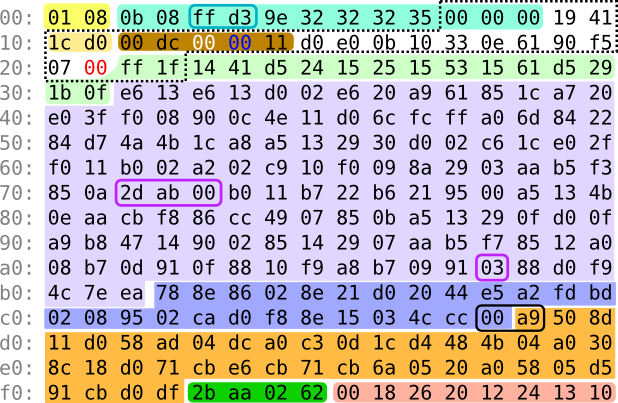
\includegraphics[width=0.8\textwidth,keepaspectratio,center]{a_mind_is_born.png}
  \caption{The annotated representation of the compiled version of A Mind Is Born, a demo by Linus Åkesson. The different color overlays highlight the meaningful regions of the program \citep{akesson_mind_2017}.}
  \label{graphic:a_mind_is_born}
\end{figure}

As a display of knowledge, the author highlights how different hexadecimal notations represent different parts of the software. Along with knowledge of how hexadecimal instructions map to the instruction set of the specific chip of of the Commodore 64 (in this case, the SID 8580), the practical use of these instructions takes productive advantage of ambivalence and side-effects\footnote{Linus Åkesson explains how he layers functionality on the same syntactical tokens: \emph{We need to tell the VIC chip to look for the video matrix at address \$0c00 and the font at \$0000. This is done by writing \$30 into the bank register (\$d018). But this will be done from within the loop, as doing so allows us to use the value \$30 for two things. An important property of this particular bank configuration is that the system stack page becomes part of the font definition}. \citep{akesson_mind_2017}}.

Demosceners therefore tend to write beautiful, deliberate code which is hardly understandable by other programmers without explanation, and yet hand-optimized for the machine. In addition to software developers' attempts to make intelligible via their source code, this practice adds a perspective on the relationship between aesthetics and understanding. Here, aesthetics do not support and enable understanding, but rather become a proof of the mastery and skill involved in crafting such a concise input for such an overwhelming output; it hints that one needs a degree of expert knowledge in order to appreciate these kinds of program texts.

Hackers are therefore programmers who write code within a variety of settings, from academia to hobbyists through professional software development, with an explicit focus on knowledge and skill. Yet, some patterns emerge. First, one can see the emphasis on the \emph{ad hoc}, insofar as choosing the right tool for the right job is a requirement for hacker code to be valued positively. This requirement thus involves an awareness of which tool will be the most efficient at getting the task at hand done, with a minimum of effort and minimum of overhead, usually at the expense of sustaining or maintaining the software beyond any immediate needs, making it available or comprehensible neither across time nor across individuals, a flavour of \emph{locality} and \emph{technical context-sensitivity}. Second, this need for knowing and understanding one's tools hints at a material relationship to code, whether instructions land in actual physical memory registers, staying away from abstraction and remaining in concrete reality by using \emph{magic numbers}, or sacrificing semantic clarity in order to \emph{"shave off"} a character or two. Throughout, there is the recurring requirement of doing the most with the least, of written parsimony leading to executed expansiveness.

Hacking therefore involves knowledge: knowledge of the hardware, knowledge of the programming language used and knowledge of the tradeoffs acceptable all the while exhibiting an air of playfulness. They tend to \emph{get the job done} and \emph{do it for the sake of doing it}, at the expense of conceptual soundness. If hacking can be considered a way of doing which deals with the practical intricacies of programming, involving concrete knowledge of the hardware and the language, they stand at the polar opposite of another community of source code practictionners. Scientists who write source code (of which computer scientists are a subset) engage with progamming first and foremost at the conceptual level, with different locii of implementation: either as a \emph{theory}, or as a \emph{model}.

\subsection{Scientists}
\label{subsec:scientists}

Historically, programming emerged as a distinct practice from the computing sciences: not all programmers are computer scientists, and not all computer scientists are programmers. Nonetheless, scientists engage with programming and source code in distinct ways, and as such open up the landscape of the type of code which can be written, as well as the standards which support the evaluation of formally satisfying code. First, we will look at code being written outside of computer science research activities and see how the specific needs of usability, replicability and data structuring link back to standards of software development. Then, we will turn to the code written by computer scientists and examine how ideal of computation manifest themselves in concrete implementations.

\subsubsection{Computation as a means}
\label{subsubsec:computation-means}

Scientific computing, defined as the use of computation in order to solve non-computer science tasks, started as early as the 1940s and 1950s in the United States, aiding in the design of the first nuclear weapons, aerodynamics and ballistics, among others \citep{oberkampf_verification_2010}. Calculations necessary to the verification of theories in disciplines such as physics, chemistry or mathematics were handed over to the computing machines of the time for faster and more correct processing. Beyond the military applications of early computer technology, the advent of computing technology would prove to be of great assistance in physics and engineering, as shown by Harlow and Fromm's article on \emph{Computer Experiments in Fluid Dynamics}\footnote{"\emph{The fundamental behavior of fluids has traditionally been studied in tanks and wind tunnels. The capacities of the modern computer make it possible to do subtler experiments on the computer alone.}" \citep{harlow_computer_1965}}, or the report on \emph{Man-Computer Symbiosis} by J.C.R. Licklider \citep{licklider_mancomputer_1960}.

The remaining issue is to make computers more accessible to scientists who did not have direct exposure to this new technology, and therefore might be unfamiliar to the intricacies of their use. While universities can afford mainframe computers so that scientists do not have to wait for the personal computer revolution, another vector for simplification and accessibility is the development of adequate programming languages. The intent is to provide non-computer scientists with easy means to instruct the computer on how to perform computations relevant to their work, ultimately aiming to situate computation as the third pillar of science, along with theorization and experimentation \citep{vardi_science_2010}.

Such an endeavour started with the BASIC\footnote{BASIC stands for Beginners' All-purpose Symbolic Instruction Code.} programming language. Developed in 1964 at Dartmouth College, it aimed at addressing this hurdle by designing "\emph{the world's first user-friendly programming language}" \citep{brooks_finally_2019}, and led the personal computer revolution by allowing non-technical individuals to write their own software. By the dawn of the 21\^{st} century, scientific computing had increased in the scope of its applications, extending beyond engineering and experimental, so-called "hard" sciences, to social sciences and the humanities. It had also incrased in the time spent developing and using software \citep{prabhu_survey_2011,hannay_how_2009}, with the main programming languages used being MATLAB, C/C++ and Python. While C and C++'s use can be attributed to their historical standing, popularity amongst computer scientists, efficiency for systems programming and speed of execution, MATLAB and Python offer different perspectives. MATLAB, originally a matrix calculator from the 1970s, became popular with the academic community by providing features such as a reliable way to do floating-point arithmetic and a friendly graphical user interface (GUI). Along with its powerful array-manipulation features, this ability to visualize large series of data and plot it on a display largely contributed to MATLAB's popularity \citep{moler_history_2020}. The combination of \ref{code:mesh_m} and \ref{graphic:mesh-visualization} shows how concise the plotting of a three-dimensional plane is in MATLAB. In the source code, it requires only one call to \lstinline{mesh}, and the output is a complete visual rendering, with reasonable and aesthetically pleasing visual default settings in the form of graded axes.

\begin{listing}
  \inputminted{matlab}{./corpus/mesh.matlab}
  \caption{Mesh.m}
  \label{code:mesh_m}
\end{listing}

\begin{figure}
  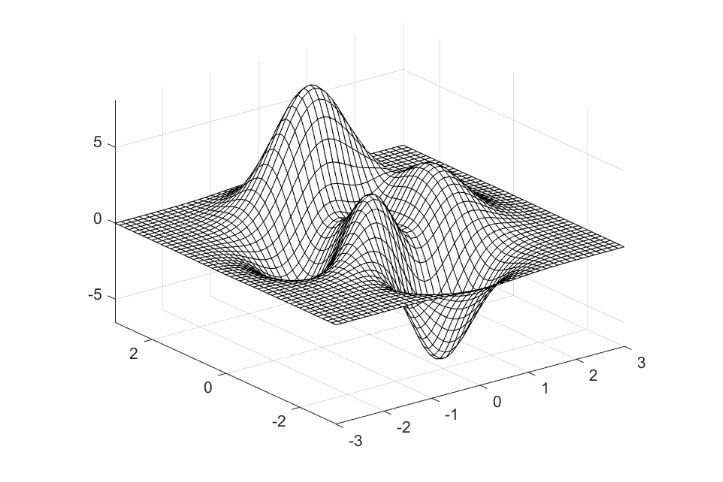
\includegraphics[width=0.8\textwidth,height=\textheight,keepaspectratio,center]{matlab.png}
  \caption{Visualization of a 3D-mesh in Matlab}
  \label{graphic:mesh-visualization}
\end{figure}

Along with MATLAB, Python represents the advent of the so-called scripting languages: programming  languages which offer readability and versatility, along with decoupling from the actual operating system that it is being executed on. System languages, such as C, are designed to interact directly with the computer hardware, and to constitute data structures from the ground up. On the other hand, scripting languages were designed and used in order to connect existing software systems or data sources together, most notably in the early days of shell scripting (such as \lstinline{Bash}, \lstinline{sed} or \lstinline{awk}, as seen in \ref{code:select_lines_awk}) \citep{ousterhout_scripting_1998}. Starting with the late 1990s, and the appearance of languages such as Perl and Python, scripting languages became more widely used by non-programmers who already had data to work with and only needed the tools to exploiThe development of additional scientific libraries such as \emph{SciKit}, \emph{NumPy} for mathematics and numerical work or \emph{NLTK} for language processing and social sciences in Python complemented the language's ease of use by providing manipulation of complex scientific concepts \citep{millman_python_2011}.

This steady rise of scientific computing has nonetheless highlighted the apparent lack of quality standards in academic software, and how the lack of value judgments on the software written might impact the reliability of the scientific output\citep{hatton_how_1994}. Perhaps the most well-known instance of poor standards in programming was revealed by the leak of the source code of the Climate Research Unit from the University of East Anglia in 2009 \citep{merali_computational_2010}. In the leak, inline comments of the authors show that particular variable values were chosen to make the simulation run, with scientific accuracy being only a secondary concern. Code reviews of external software developers point out to the code of the CRU leak as being a symptom of the general state of academic software\footnote{Professor Darrel Ince stated to the UK Parliamentary Committee in February 2010: "\emph{There is enough evidence for us to regard a lot of scientific software with worry. For example Professor Les Hatton, an international expert in software testing resident in the Universities of Kent and Kingston, carried out an extensive analysis of several million lines of scientific code. He showed that the software had an unacceptably high level of detectable inconsistencies.}" \citep{committee_disclosure_2010}}.

In response, the beginning of the 2000s has seen the desire to re-integrate the best practices of software engineering in order to correct scientific software's lack of accuracy, resulting in the formation of communities such as the Research Software Engineers\citep{woolston_why_2022}. As we have seen above, software engineering had developed on their own since its establishment as an independent discipline and professional field. Such a split, described by Diane Kelly as a "\emph{chasm}" \citep{kelly_software_2007} then had to face the different standards to which commercial software and scientific software were held to. For instance, commercial software must be extensible and performant, two qualities that do not necessarily translate to an academic setting, in which software might be written within a specific, time-constrained, research project, or in which access to computing resources (i.e. supercomputers) might be less of a problem.

It seems that software's position in the scientific inquiry is no longer that of a helpful crutch, but rather of an inevitable step. Within Landau et. al's conception of the scientific process as the progression from problem to theory, followed by the establishment of a model, the devising of a method, and then on to implemementation and finally to assessment \citep{landau_survey_2011}, code written as academic software is involved in the latter two stages of  method and implementation. As such, it has to abide by the processes and requirements of scientific research. First and foremost, reproducibility is a core requirement of scientific research in general and bugs in a scientific software system can lead to radically different ouptuts given slightly different input data, while concealing the origin of this difference, and compromising the integrity of the research and of the researcher. Good academic code, then, is one which defends actively against these, perhaps to the expense of performance and maintainability. This can be addressed by reliable error-handling, regular assertions of the state of the processed data and extensive unit testing \citep{wilson_best_2014}.

Furthermore, a unique aspect of scientific software comes from the lack of clear upfront requirements. Such requirements, in software development, are usually provided ahead of the programming process, and should be as complete as possible. As the activity of scientists is defined by an incomplete understanding of the application domain, requirements tend to emerge as further knowledge is developed and acquired \citep{segal_when_2005}. As a result, efforts have been made to familiarize scientists with software development best practices, so that they can implement quality software on their own. Along with field-specific textbooks\footnote{See \emph{Effective Computation in Physics} \citep{scopatz_effective_2015} or \emph{A Primer for Computational Biology} \citep{oneil_primer_2019} covering similar software-oriented material from different academic perspectives.} the most prominent initiative in the field is \emph{Software Carpentry}, a collection of self-learning and teaching resources which aims at implementing software best practices across academia, for scientists and by scientists. Founded by Greg Wilson, the co-editor of \emph{Beautiful Code}, the organization's title refers directly to equivalents in the field of software development.

We see a convergence of quality standards of broad academic software towards the quality standards of commercial software development. Meanwhile, computer science worked towards asserting and pursuing its own field of research, sometimes distinct from the discipline of programming. Unlike other scientific fields possesses its own specific standards of programming, taking software not as a means to an end, but as the end itself.

\subsubsection{Computation as an end}
\label{subsubsec:computation-end}

Computer scientists are scientists whose work focuses on computation as an object, rather than as a tool. They study the phenomenon of computation, investigating its nature and effects through the development of theoretical frameworks around it. Originally derived from computability theory, as a branch of formal mathematical logic, computation emerged as an autonomous field from work in mechanical design and configuration, work on circuit and language design, work on mathematical foundations, information theory, systems theory and expert systems, computer science establishes its institutional grounding with the inauguration of the first dedicated academic department at Purdue University in 1962 \citep{ifrah_universal_2001}.

From this multifaceted heritage and academic interdisciplinarity, computer scientists identified key areas such as data structures, algorithms and language design as foundations of the discipline \citep{wirth_algorithms_1976}. Thoughout the process of institutionalization, the tracing of the "roots" of computation remained a constant debate as to whether computer science exists within the realm of mathematics, of engineering or as a part of the natural sciences. The logico-mathematical model of computer science contends that one can do computer science without an electronic computer, while the engineering approach of computer science tends to put more practical matters, such as architecture, language design and systems programming (implicitly assuming the use of a digital computer) at the core of the discipline; both being a way to generate and process information as natural phenomenon \citep{tedre_development_2006}.

The broad difference we can see between these two conceptions of computer science is that of \emph{episteme} and \emph{techne}. On the theoretical and scientific side, computer science is concerned with the primacy of ideas, rather than of implementation. The quality of a given program is thus deduced from its formal (mathematical) properties, rather than its formal (aesthetic) properties. The first manifestations of such a theoretical focus can be found in the Information Processing Language in 1956 by Allen Newell, Cliff Shaw and Herbert Simon, which was originally designed and developed to prove Bertrand Russell's \emph{Principia Mathematica} \citep{ifrah_universal_2001}. While the IPL, as one of the very first programming languages, influenced the development of multiple subsequent languages, in particular some later languages came to be known as logic programming languages. These are based on a formal logic syntax of facts, rules and clauses about a given domain and whose correctness can be easily proven. We can see in \ref{code:prolog_sample} an example of the \emph{Prolog} logic programming language. Its syntax appears very repetitive, a result of the few keywords used (\lstinline{induce}, \lstinline{element} and \lstinline{clause}), and drawing directly from the lexical field of logic and framing the problem domain. Due to its Turing-completeness, one can write in Prolog programs such as language processing, web applications, cryptography or database programming, but its use seems to remain limited outside of theoretical circles in 2021, according to the Stackoverflow Developer survey for popular language uses \citep{stackoverflow_stack_2021}.

\begin{listing}
  \inputminted{prolog}{./corpus/inductive.pl}
  \caption{The Prolog programming language focuses first and foremost on logic predicates in order to perform computation, rather than more practical system calls.}
  \label{code:prolog_sample}
\end{listing}

Lisp—\emph{LISt Processor}— is another programming language which shares this feature of theoretical soundness faced with a limited range of actual use in production environments. It was developed in 1958, the year of the Dartmouth workshop on Artificial Intelligence, by its organizator, John McCarthy, and was designed to process lists. Inheriting from IPL, it retained the core idea that programs should separate the knowledge of the problem (input data) and ways to solve it (internal rules), assuming that the rules are independent to a specific problem.

The base structural elements of Lisp are not symbols, but lists (of symbols, of lists, of nothing), and they themselves act as symbols (e.g. the empty list). By manipulating those lists recursively—that it, processing something in terms of itself—Lisp highlights even further this tendency to separate computation from the problem domain, exhibiting autotelic tendencies. This is facilitated by its atomistic and relational structure: in order to solve what it has do, it evaluates each symbol and traverses a tree-structure in order to find a terminal symbol. Building on these features of complex structures with simple elements, Willam Byrd, computer scientst at the University of Utah, describes the Scheme interpreter written in Scheme\footnote{Scheme is a Lisp dialect, designed a few years after Lisp itself, and also at MIT.} shown in (\ref{code:scheme_interpreter}) as "\emph{the most beautiful program ever written}" \citep{byrd_william_2017}.

\begin{listing}
  \inputminted{scheme}{./corpus/interpreter.scheme}
  \caption{Scheme interpreter written in Scheme, revealing the power and self-reference of the language.}
  \label{code:scheme_interpreter}
\end{listing}

The beauty of such a program, for Byrd, is the ability of these fourteen lines of source cede to reveal powerful and complex ideas about the nature and process of computation. As an interpreter, this program can take any valid Scheme input and evaluate it correctly, recreating computation in terms of itself. It does so by showing and using ideas of recursion (with calls to \lstinline{eval-expr}), environment (with the evaluation of the \lstinline{body}) and lambda functions, as used throughout the program. Byrd equates the feelings he experiences in witnessing and pondering the program above to those suggested by Maxwell's equations, which constitute the foundation of classical electromagnetism (see \ref{graphic:maxwell-equations}), a comparison that other computer scientists have made \citep{kay_conversation_2004}. In both cases, the quality ascribed to those inscriptions come from the simplicity and conciseness of their base elements—making it easy to understand what the symbols mean and how we can compute relevant outputs—all the while allowing for complex and deep  consequences for, respectively, computer science and electromagnetism.

\begin{figure}
  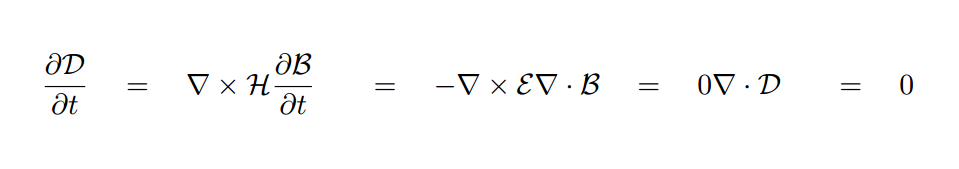
\includegraphics[width=0.8\textwidth,height=\textheight,keepaspectratio,center]{maxwell.png}
  \caption{Maxwell's equations form a terse, unified basis for electromagnetism, optics and electric circuitry.}
  \label{graphic:maxwell-equations}
\end{figure}

With this direct manipulation of symbolic units upon which logic operations can be performed, Lisp became the language of AI, an intelligence conceived first and foremost as abstractly logical. Lisp-based AI was thus working on what Seymour Papert has called "toy problems"—self-referential theorems, children's stories, or simple puzzles or games \citep{nilsson_early_2009}. In these, the problem and the hardware are reduced from their complexity and multi-consequential relationships to a finite, discreete set of concepts and situations. Confronted to the real world—that is, to commercial exploitation—Lisp's model of symbol manipulation, which proved somewhat successful in those early academic scenarios, started to be applied to issues of natural language understanding and generation in broader applications. Despite disappointing reviews from government reports regarding the effectiveness of these AI techniques, commercial applications flourished, with companies such as Lisp Machines, Inc. and Symbolics offering Lisp-based development and support. Yet, in the 1980s, over-promising and under-delivering of Lisp-based AI applications, which often came from the combinatorial explosion deriving from the list- and tree-based representations, met a dead-end. In this case, a restricted problem domain can enable a particular aesthetic judgment, but also exclude others.

"\emph{By making concrete what was formerly abstract, the code for our Lisp interpreter gives us a new way of understanding how Lisp works}", notes Michael Nielsen in his analysis of Lisp, pointing at how, across from the \emph{episteme} of computational truths stands the \emph{techne} of implementation \citep{nielsen_lisp_2012}. The alternative to such abstract, high-level language, is then to consider computer science as an engineering discipline, a shift between theoretical programming and practical programming is Edsger Dijkstra's \emph{Notes on Structured Programming}. In it, he points out the limitation of considering programming exclusively as a concrete, bottom-up activity, and the need to formalize it in order to conform to the standards of mathematical logical soundness. Dijkstra argues for the superiority of formal methods through the need for a sound theoretical basis when writing software, at a time when the software industry is confronted with its first crisis.

Within the software engineering debates, the theory and practice distinction had a slightly different tone, with terms like “art” and “science” labeling two, implicitly opposed, perspectives on programming. Programming suffered from an earlier image of an inherently unmanageable, unsystematic, and artistic activity, , many saw programming essentially as an art or craft \citep{tedre_development_2006}, rather than an exact science. Beyond theoretical soundness, computer science engineering concerns itself with quantified efficiency and sustainability, with measurements such as the \emph{O()} notation for program execution complexity. It is not so much about whether it is possible to express an algorithm in a programming language, but whether it is possible to run it effectively, in the contingent environments of hardware, humans and problem domains\footnote{Notably, algorithms in textbooks tend to be erroneous when used in production; only in five out of twenty are they correct \citep{pattis_textbook_1988}.}.

This approach, halfway between science and art, is perhaps best seen in Donald Knuth's magnum opus, \emph{The Art of Computer Programming}. In it, Knuth summarizes the findings and achievements of the field of computer science in terms of algorithm design and implementation, in order to "\emph{to organize and summarize what is known about the fast subject of computer methods and to give it firm mathematical and historical foundations.}" \citep{knuth_art_1997}. The art of computer programming, according to him, is therefore based on mathematics, but differs from it insofar as it does have to deal with concepts of effectiveness, implementation and contingency. In so doing, Knuth takes on a more empirical approach to programming than his contemporaries, inspecting source code and running software to assess their performance, an approach he first inaugurated for FORTRAN programs when reporting on their concrete effectiveness for the United States Department of Defense \citep{defensetechnicalinformationcenter_dtic_1970}.

Another influential textbook insisting that computation is not to be seen as an autotelic phenomenon is \emph{Structure and Interpretation of Computer Programs}. In it, the authors insist that source code is "\emph{must be written for people to read, and only incidentally for machines to execute}" \citep{abelson_structure_1979}. Readability is thus an explicit standard in the discipline of programming, along with a less visible focus on efficiency and verifiability. Finally, the aesthetic standard in this more engineering approach to computer science is, again, proportionality between the number of lines of code written and the complexity of the idea explained. We can see such a value at play in the series \emph{Beautiful Julia Algorithms} \citep{moss_beautifulalgorithms_2022}. For instance, \ref{code:bubble_sort_julia} implements the classic Bubble Sort sorting algorithm in one loop rather than the usual two loops in C, resulting in an easier grasping of the concept at hand, rather than being distracted by the idiosyncracy of the implementation details. The simplicity of scientific algorithms is expressed even further in \ref{code:nearest_neighbor_julia} the one-line implementation of a procedure for finding a given element's nearest neighbor, a crucial component of classification systems.

\begin{listing}
  \inputminted{julia}{./corpus/bubblesort.jl}
  \caption{Bubble Sort implementation in Julia uses the language features to use only a single iteration loop. \citep{moss_bubblesort_2021}}
  \label{code:bubble_sort_julia}
\end{listing}

\begin{listing}
  \inputminted{julia}{./corpus/nearest_neighbor.jl}
  \caption{Nearest neighbor implementation in Julia \citep{moss_nearestneighbors_2021}.}
  \label{code:nearest_neighbor_julia}
\end{listing}

According to Tedre, computer science itself was split in a struggle between correctness and productivity, between theory and implementation, and between formal provability and intuitive art \citep{tedre_science_2014}. In the early developments of the field, when machine time was expensive and every instruction cycle counted, efficiency ruled over elegance, but in the end he assesses elegance prevailed, a concept we will explore further in \ref{subsec:lexical-fields}.

In closing, one should note that the \emph{Art} in the title of Knuth's series does not, however, refer to art as a fine art, or a purely aesthetic object. In a 1974 talk at the ACM, Knuth goes back to its Latin roots, where we find \emph{ars}, \emph{artis} meaning "skill.", noting that the equivalent in Greek being τεχνη, the root of both "technology" and "technique.". This semantic proximity helps him reconcile computation as both a science and an art, the first due to its roots in mathematics and logic, and the second

\begin{quote}
  because it applies accumulated knowledge to the world, because it requires skill and ingenuity, and especially because it produces objects of beauty. A programmer who subconsciously views himself as an artist will enjoy what he does and will do it better. Therefore we can be glad that people who lecture at computer conferences speak about the state of the Art. \citep{knuth_computer_1974}
\end{quote}

When written within an academic and scientific context, source code tends to align with the aesthetic standards of software development, valuing reliability, reabability, sustainability, for instance through Greg Wilson's work on the development of software development principles through the Software Carpentry initiative. This alignment can also be seen in a conception of computer science as a kind of engineering, as an empirical practice which can and should still be formalized in order to become more efficient. There, one can turn to Donald Knuth's \emph{Art of Computer Programming} to see the connections between the academia's standards and the industry's standards.

And yet, a conception of computation as engineering isn't the only conception of computer science. Within a consideration of computer science as a  theoretical and abstract object of study, source code becomes a means of providing insights into more complex abstract concepts, seen in the Lisp interpreter, or one-line algorithms implementing foundational algorithms in computer science. The beauty of scientific source code is thus associated with the beauty of other sciences, such as mathematics and engineering. And yet, Knuth is also known as the advocate of literate programmig, a practice which engages first source code as a textual, rather than scientific, object. To address this nature, we complete our overview of code practitioners by turning to the software artists, who engage most directly with program texts through source code poetry.

\subsection{Poets}
\label{subsec:poets}

Ever since Christopher Stratchey's love letters, programmers have been curious of the intertwining of language and computation. Electronic literature is a broad field encompassing natural language texts taking full advantage of the dynamic feature of computing to redefine the concept of text, authorship and readership. It encompasses a variety of approaches, including generative literature, interactive fiction, visual poetry, source code poetry and esoteric programming languages, as well as certain aspects of software art. Here, we focus here only on the elements of electronic literature which shift their focus from output to input, from executable binary with transformed natural language as a result, to static, latent source Particularly, we pay attention to the role of function, correctness and meaning-making in these particular program texts.

\subsubsection{Code poetry as executed literature}

Electronic literature, a form based on the playful \emph{détournement} of the computer's constraints, gets closer to our topic insofar as the poems generated represent a more direct application of the rule-based paradigm to the syntactical output of the program. Starting in 1953 with Christopher Stratchey's love letters, generated (and signed!) by MUC, the Manchester Univac Computer, computer poems are generated by algorithmic processes, and as such rely essentially on this particular feature of programming: laying out rules in order to synthesize syntactically and semantically sound natural language poems. Here, the rules themselves matter only in relation to the output, as seen by their ratio: a single rule for a seemingly-infinite amount of outputs, with these outputs very often being the only aspect of the piece shown to the public.

These works and their authors build on a longer tradition of rule-based composition, from Hebrew to the Oulipo and John Cage's indeterministic composition, amongst others \citep{cramer_words_2003}, a tradition in which creativity and beauty can emerge from within a strict framework of formal rules. Nonetheless, the source code to these works is rarely released in conjunction with their output, hinting again at their lesser importance in terms of their overall artistic values. If electronic literature is composed of two texts, a natural-language output and a computer-language source, only the former is actually considered to be poetry, often leaving the latter in its shadow (as well as, sometimes, its programmer, an individual sometimes different from the poet). The poem exists through the code, but isn't exclusively limited to the human-readable version of the code, as it only comes to life and can be fully appreciated, under the poet's terms, once interpreted or compiled. While much has been written on electronic literature, few of those commentaries focus on the soundness and the beauty of the source code as an essential component of the work, and only in recent times have we seen the emergence of close-readings of the source of some of these works for their own sake \citep{montfort_10_2014,marino_critical_2020,brock_rhetorical_2019}. These constitute a body of work centered around the concept of generative aesthetics \citep{goriunova_read_2005}, in which beauty comes from the unpredictable and somewhat complex interplay of rule-based systems, and whose manifestations encompass not only written works, but games, visual and musical works as well.

Source code poetry is thus a form of electronic literature, but also a form of  software art. Software art is an umbrella term regrouping artistic practices which engage with the computer on a somewhat direct, material level, whether through hardware\footnote{See Alexei Shuglin's \emph{386 DX} (1998-2013)} or software\footnote{See Netochka Nezanova's \emph{Nebula.M81} (1999)}. This space for artistic experimentation flourished at the dawn of the 20th century, with initiatives such as the \emph{Transmediale} festival's' introduction of a \emph{software art} award between 2001 and 2004, or the \emph{Run\_me} festival, from 2002 to 2004. In both of these, the focus is on projects which incorporate standalone programmes or script-based applications which aren not merely functional tools, but also act as an effective artistic proposition, as decided by the artist, jury and public. These works often bring the normally hidden, basic materials from which digital works are made (e.g. code, circuits and data structures) into the foreground \citep{yuill_code_2004}. From this perspective, code poetry is a form a software art where execution is required, but not sufficient to constitute a meaningful work.

The approach of code poets is therefore more specific than broad generative aesthetics: it is a matter of exploring the expressive affordances of source code, and the overlap of machine-meaning and human-meaning, acting as a vector for artistic communication. Such an overlap of meaning is indeed the specific feature of source code poetry. In a broad sense, code poetry conflates classical poetry (as strict syntactical and phonetical form, combined with poetic expressivity) with computer code, but it is primarily defined by its inversion of the reading and executing processes. Usually, a program text is loosely assumed to be somewhat pleasurable to read, but is expected to be executable. Code poems rather assume that the program text is somewhat executable, but demand that it is pleasurable to read. Following the threads laid out by electronic literature, code poetry starts from this essential feature of computers of working with strictly defined formal rules, but departs from it in terms of utility. Code poems are only functional insofar as they are accepted by the intepreter or compiler of the language in which they are written, but they are functional nonetheless. The are functional to the computer, in that they are composed in a legal syntax and can be successfully parsed; but they do not need their output to do anything of immediate and measurable \emph{use}. Such formal compliance is only a pre-requisite, a creative constraint, for their human writers.

Within this reliance on creative constraints provided by a computing environment, the emphasis here is on the act of reading, rather than on the act of deciphering, as we have seen with obfuscated code (and in functional code in general). Source code poems are often easy to read, and have an expressive power which operates beyond the common use of programming. They also make the reader reconsider the relationship to the machine, and the relationship to function. By using a machine language in the way the machine expects to receive it, it is no longer software referring to itself, exploring its own poetics and its specific meaning-making abilities. By forcing itself to be functional—that is, to produce meaningful output as the result of execution, it becomes software investigating itself, and through that, investigating the system within which it exists and acts, and the assumptions we ascribe to it. Code poems thus shed a new light on how and why source code is written, not as a functional artefact, but as a poetic one, focusing on fabrication rather than production, and expressing a subject rather than an intent \citep{paloque-berges_poetique_2009}.

In their different manifestations, code poems make the boundary between computer meaning and human meaning thinner and thinner, a feature often afforded by the existence and use of higher-level programming languages. Starting with the development of FLOWMATIC in 1955 by Grace Hopper, it was shown that an English-like syntactical system could be used to communicate concepts for the computer to process. From there, programming languages could be described along a gradient, with binary at the lowest end, and natural language (in an overwheling majority, English) at the highest end. This implies that they could be written and read similarly to English, including word order, pronouncation and interpretation, similar to the error-tolerance of human laguages, which doesn't cause the whole communication process to fail whenever a specific word, or a word order isn't understood.

\subsubsection{Layered machine texts}
\label{subsubsec:layered-machine-texts}

Yet, code poems from the 20th century aren't the first time where a part of the source code is written exclusively to elicit a human reaction, without any machinic side-effects. One of the earliest of those instances is perhaps the Apollo 11 Guidance Computer (AGC) code, written in 1969 in Assembly \citep{garry_lunar_1969}. Cultural references and jokes are peppered throughout the text as comments, asserting computer code as a means of expression beyond exclusively technical tasks\footnote{Other files include comments such as "Crank that wheel" or "Burn Baby Burn" when triggering the ignition subroutine.}, and independent from a single writer's preferences, since they passed multiple checks and review processes to end up in the final, submitted and executed document, such as reproduced in \ref{code:numero_mysterioso_asm}.

\begin{listing}
  \inputminted{ca65}{./corpus/numero_mysterioso.asm}
  \caption{AGC source code for the Lunar Landing Guidance Equation, 1969}
  \label{code:numero_mysterioso_asm}
\end{listing}

Code comments allow a programmer to write in their mother tongue, rather than in the computer's, enabling more syntactic and semantic flexibility, and thus reveal a burgeoning desire for programmers to express themselves within their medium of choice, in the midst of an impersonal interaction with the machine system.

Rather than limiting their lexical field to comments, some writers decided to engage directly with machine keywords in order to compose poems. One of the first instances of this human poetry composed with machine syntax are the Poèmes Algol by Noël Arnaud \citep{arnaud_poemes_1968}. As a member of the Oulipo movement, he sets himself the constraints of only using those reserved keywords of the ALGOL 68 programming language to extract meaning beyond their original purpose. Reading those, one is first struck by their playfulness in pronounciation, and subsequently by the unexpected linguistic associations that they suggest.

More recently, this has been illustrated in the work of MOONBIT \citep{mosteirin_moonbit_2019}, a series of code poems computationally extracted from the AGC's source code, with those two program texts standing almost 50 years apart. In their work, the authors want to highlight that software is not only functional, but also social, political and aesthetic; importantly, the relation between aesthetics and function is not seen as mutually exclusive, but rather as supplementary\footnote{"\emph{The aesthetic features of computer code—often characterized by a rigidly formal, restricted syntax, and numerous paralinguistic dimensions—sometimes have a supplemental character; they appear, at times, almost ornamental in their sheer excess beyond the functional elements and programmed goals. At other times, these features are an intrinsic and necessary part of the code. We believe that these special properties of computer code make possible imaginative uses or misuses by its human programmers and that these properties and features justify our exuberant readings, misreadings, translations, and appropriations.}" \citep{mosteirin_moonbit_2019}}. As programmers could already express themselves in a language as rigid as Assembly, subsequent programming languages would further expand poetic possibilities.

Code poetry benefited greatly from the advent of scripting languages, such as Python, Ruby or Perl (see \ref{subsec:scientists} above). As we've seen, scripting languages are readable and versatile; readable because their syntax tends to borrow from natural languages rather than invented idioms, at the expense of functionality\footnote{For instance, C's \lstinline{strtok()} separates a string of text in a list of strings along several particular delimiters, while Python's \lstinline{str.split()} does the same thing with a more readable name, but with only one delimiter.}, and versatile because they often handle some of the more complex and subtle data and platform idiosyncracies\footnote{Python and Perl are both dynamically typed languages, meaning that the writer does not need to bother with additional syntax and possible verbosity, but rather focus only on the most expressive tokens, all while letting the interpreter deal with the kinds of errors which would undermine the functionality requirement of code poetry in other languages.}.

The community of programmers writing in Perl, \emph{perlmonks}\footnote{See their website: \url{https://perlmonks.org/}, with the spiritual, devoted and communal undertones that such a name implies.} has been one of the most vibrant and productive communities when it comes to code poetry. This particular use of Perl started in 1990, when the language creator Larry Wall shared some of the poems written in the language, and it gained further exposition through the work of Shannon Hopkins \citep{hopkins_camels_1992}. The first Perl poem is considered to have been written by Wall in 1990, reproduced in \ref{code:japh_perl}.

\begin{listing}
  \inputminted{perl}{./corpus/japh.pl}
  \caption{Just Another Perl Hacker, japh.pl}
  \label{code:japh_perl}
\end{listing}

Hopkins analyzes the ability of the poem to enable dual understandings of the source—human and machine. Yet, departing from the previous conceptions of source that we have looked at, code poetry does not aim at expressing the same thing to the machine and to the human. The value of a good poem comes from its ability to evoke different concepts for both readers of the source code. As Hopkins puts it:

\begin{quote}
  In this poem, the q operator causes the next character (in this case a newline) to be taken as a single quote, with the next occurrence of that delimiter taken as the closing quote. Thus, the single-quoted line 'Just another Perl hacker' is printed to STDOUT. In Perl, the "unless \$spring" line is mostly filler, since \$spring is undefined. In poetical terms, however, "\$spring" is very important: haiku poetry is supposed to specify (directly or indirectly) the season of the year. As for the q operator, that reads in English as the word "queue", which makes perfect sense in the context of the poem. \citep{hopkins_camels_1992}
\end{quote}

The poem \emph{Black Perl}, submitted anonymously in 1990, is another example of the richness of the productions of this community. It is presented in \ref{code:black_perl} in its updated form by kck, making it compatible for perl 5.20 in 2017. The effort of Perl community members of updating Black Perl to more recent versions of the language is a testament to the fact that one of the intrinsic qualities of the poem is its ability to be correctly processed by the language interpreter.

\begin{listing}
  \inputminted{perl}{./corpus/black_perl.pl}
  \caption{Black Perl is one of the first Perl poems, shared anonymously online. It makes creative use of Perl's flexible and high-level syntax.}
  \label{code:black_perl}
\end{listing}

The most obvious feature of this code poem is that it can be read by anyone, including by readers with no previous programming experience: each word is valid both as English and as Perl. A second feature is the abundant use of verbs. Perl belongs to a family of programming languages grouped under the \emph{imperative} paradigm, which matches a grammatical mood of natural languages, the \emph{imperative mood}. Such mood emphasizes actions to be take rather than, for instance, descriptions of situations, and thus sets a clear tone for the poem. The fact that Perl is based on stating procedures to be executed and states to be changed creates this feeling of relentless urgency when reading through the poem, a constant need to be taking actions, for things to be changed. Here, the native constraints of the programming language interacts directly with the poetic suggestion of the work in a first way: the nature of Perl is that of giving orders, resulting in a poem which addresses \emph{someone} to execute \emph{something}. Still, Perl's flexibility leaves us wondering as to who and what are concerned by these orders. Is the poem directing its words to itself? To the reader? Is Perl just ever talking exclusively to the computer? This ambiguity of the adressee adds to the ominousness of each verse.

The object of each of these predicates presents a different kind of ambiguity: earlier versions of Perl function in such a way that they ignore unknown tokens\footnote{e.g. undefined variables do not cause a core dump.}\footnote{Which results in the poem having to be updated/ported, in this case by someone else than the original writer}. Each of the non-reserved keywords in the poem are therefore, to the Perl interpreter, potentially inexistant, allowing for a large latitude of creative freedom from the writer's part. Such a feature allows for a tension between the strict, untoucheable meaning of Perl's reserved keywords, and the almost infinite combination of variable and procedure names and regular expressions. This tension nonetheless happens within a certain rhythm, resulting from the programming syntax: \lstinline{kill them, dump qualms, shift moralities}, here alternating the computer's lexicon and the poet's, both distinct and nonetheless intertwined to create a \emph{Gestalt}, a whole which is more than the sum of its parts.

A clever use of Perl's handling of undefined variables and execution order allows the writer to use keywords for their human semantics, while subverting their actual computer function. For instance, the \lstinline{die} function should raise an exception, but wrapped within the \lstinline{exit ()} and \lstinline{close} keywords, the command is not interpred and therefore never reaches the execution point, bypassing the abrupt interruption. The subversion here isn't purely semiotic, in the sense of what each individual word means, but rather in how the control flow of the program operates—technical skill is in this case required for artistic skill to be displayed.

Finally, the use of the \lstinline{BEFOREHAND:} and \lstinline{AFTERWARDS:} words mimick computing concepts which do not actually exist in Perl's implementation: the pre-processor and post-processor directives. Present in languages such a C, these specify code which is to be executed respectively before and after the main routine. In this poem, though, these patterns are co-opted to reminisce the reader of the prologue and epilogue sometimes present in literary texts. Again, these seem to be both valid in computer and human terms, and yet seem to come from different realms.

This instance of Perl poetry highlights a couple of concepts that are particularly present in code poetry. While it has technical knowledge of the language in common with obfuscation, it departs from obfuscated works, which operate through syntax compression, by harnessing the expressive power of semiotic ambiguity, giving new meaning to reserved keywords. Such an ambiguity is furthermore bi-directional: the computing keywords become imbued with natural language significance, bringing the lexicon of the machine into the realm of the poetic, while the human-defined variable and procedure names, and of the regular expressions, are chosen as to appear in line with the rhythm and structure of the language. Such a work highlights the co-existence of human and machine meaning inherent to any program text\footnote{Except perhaps those which deal exclusively with scientific and mathematical concepts}.

Following in the footsteps of the \emph{perlmonks}, additional communities around code poetry have formed, whether in university settings, such as Stanford's Code Poetry Slam, which ran between 2014 and 2016 \citep{kagen_code_2016}, or as independent intiatives, like the Source Code Poetry event, which runs annual contests \citep{unknown_source_2017}. The simple constraint and low barrier to entry also results in collective writings where programmers engage in playful writing, such as in the \lstinline{#SongsOfCode} trend on a micro-blogging website where the challenge. In \ref{code:prince_java}, we can see a simple example of translation from the problem of popular pop songs into machine language. The tension between the familiarity of the song and the estrangeness of the Java syntax is a kind of puzzle that is also reminiscent of hackers, further establishing cognitive complexity as a factor in the aesthetic judgment of source code poetry.

\begin{listing}
  \inputminted{perl}{./corpus/prince.java}
  \caption{\#SongsInCode is an example of functional source code poetry written to represent the tradionally non-functional domain of pop songs.}
  \label{code:prince_java}
\end{listing}

We saw in \ref{subsec:software-developers} that the transition of programming from an annex practice to a full-fledged discipline and profession resulted in source code being recognized as a text in its own, to which engineering and artistic attention should be paid. No longer a transitional state from formula to binary, it becomes a semantic material, whose layout, organization and syntax are important to the eyes of its writers and readers. Pushing further into the direction of the visual layout of the code, such an endeavour becomes pursued for its own sake, existing parallel to the need for a program to be functional, and echoing the practice of Guillaume Apollinaire's \emph{calligrammes}.

There, the physical layout of the program text comes to the forefront, along with its executed representation. Written by Kerr and Holden in 2014, \lstinline{water.c} is a poem written in C which illustrate both of these components. In \ref{code:water_c}, we can see that the way the whitespace is controlled in the source code evokes a visual representation of water as three columns composed of ;, \{ and \{ characters, computer-understood punctuation which nonetheless holds only a tiny semantic load as block and statement delimiters.

\begin{listing}
  \inputminted{perl}{./corpus/water.c}
  \caption{water.c has a very deliberate layout and syntax, reminiscing of \emph{calligrames} \citep{holden_code_2016}.}
  \label{code:water_c}
\end{listing}

Once compiled and executed, \lstinline{water.c} gains an additional quality: its output represents moving droplets running across the screen, with a particular frame shown in \ref{code:water_out}. We see that code poetry, like other forms of writing program texts, differ from other means of expression in their dual representatiom, as source and software, static and dynamic.

\begin{listing}
  \inputminted{perl}{./corpus/water.out}
  \caption{The output of \ref{code:water_c} consists in ASCII representation of water droplets, bearing a family resemblance to BASIC one liners, and suggesting a complementary representation of water.}
  \label{code:water_out}
\end{listing}

Code poetry values code which, while being functional, expresses more than what it does, by allowing for \emph{Sprachspiele}, languages games where pronounciation, syntax and semantics are playfully composed into a fluid linguistic construct in order to match a human poetic form, such as the haiku, or to constitute a specific puzzle. A subtle interplay of human meaning and machine meaning, layout and execution allows for a complex poetic emergence.

\spacer

From engineers to poets, this section has shown how the set of individuals who write and read code is heterogeneous, varying in practices, problems and approaches. While none of these communities of practice are mutually exclusive—a software developer by day can hack on the weekend and participate in code poetry events—, they do help us grasp how source code's manifestations in program texts and its evaluation by programmers can be multifaceted. For instance, software engineers prefer code which is modular, modifiable, sustainable and understandable by the largest audience of possible contributors, while hackers would favor conciseness over expressivity, and tolerate playful idiosyncracy for the purpose of immediate, functional efficiency, with a practical engagement with the tools of their trade. On the other hand, scientific programming favors ease of use and reproducibility, along with a certain quest to represent the elegant concepts of computer science, while code poets explore the semantic tension between a human interpretation and the machine interpretation of a given source code, via syntactic games, graphical layouts and interplay between the static and executed versions of software.

Still, there are strands of similarity within this apparent diversity. The code snippets in this section show that there is a tendency to prefer a specific group of qualities—readability, conciseness, clarity, expressivity and functionality—even though different types of practices would put a different emphasis on each of those aspects. The question we turn to next, then, is to what extent do these different practices of code writing and reading share common judgments regarding their formal properties?  To start this investigation, we first analyze programmers' discourses in \ref{sec:ideals-beauty} in order to identify concrete categories of formal properties which might enable a source code to be positively valued for its appearance, before we examine the aesthetic domains code practitioners refer to when discussing beautiful code in \ref{sec:aesthetic-domains} to further qualifies these properties.

\section{Ideals of beauty}
\label{sec:ideals-beauty}

Following our overview of the varieties of practices and program texts amongst those who read and write source code, we now analyze more thoroughly what are the aesthetic standards most value by those different groups. The aim here is to formalize our understanding of which source code is considered beautiful, and to do so in a dual approach. The goal here is to capture both the specific manifestations of beautiful code as specified and enunciated by programmers, as well as the semantic contexts from which these enunciations originate. To do so, we will introduce a discourse analysis framework for the empirical study of the corpus, followed by an examination of the discourses that programmers deploy when it comes to explicit their aesthetic preferences of source code. What we will see is that a set of aesthetic values and a set of aesthetic manifestations prove to be recurringly consistent; conversely, the aesthetic domains that are mobilized to justify these values are clearly distinct.

\subsection{Introduction to the Methodology}
\label{subsec:ideals-methodology}

Discourse consists of text, talk and media, which express ways of knowing the world, of experiencing and valuing the world. This study builds on Kintsch and Van Dijk's work on providing tools to analyze an instance of discourse, and is centered around what is said to constitute good source code. While discourse analysis can also be used critically by unearthing which value judgments that occur in power relationships \citep{mullet_general_2018a}, we focus here on aesthetic value judgments, as their are first expressed through language. Of all the different approaches to discourse, the one we focus on here is that of \emph{pragmatics}, involving the spatio-temporal and intentional context in which the discourse is uttered. We find this approach particularly fitting through its implication of the \emph{cooperative principle}, in which utterances are ultimately related to one another through communicative cooperation to reveal the intent of the speaker \citep{schiffrin_approaches_1994}. Practically, this means that we assume the position of programmers talking to programmers is cooperative insofar as both speaker and listener want to achieve a similar goal: expliciting what writing good code entails. This double understanding—focusing first and foremost on utterances, and then re-examining them within a broader cooperative context—will lead us to encompass a variety of production media (blog post, forums, conferences, text books), in order to depict the cultural background (software practices as outlined above as well as additional factors such as skill levels). Our comprehension of those texts, then, will be set in motion by a a dual movement between local, micro-units of meaning and broader, theoretical macro-structure of the text, and linked by acts of co-reference \citep{kintsch_model_1978}. As the macro structure represents a certain kind of world situation, we will connect these to specific aesthetic fields, considering that the world of the aesthetics of source code is pragmatically connected, by the programmers and via their discourses, to adjacent world of the aesthetics of architecture, literature and mathematics. 

Particular attention will be paid to the difference between intentional and extensional meaning \citep{dijk_strategies_1983}. As we will see, some of the texts in our corpus tend to address a particular problem (e.g. on forums, social media or question \& answer platforms), or to discuss broader concepts around well-written code. Particularly, figures of speech such as metaphorical devices may attract attention to important concepts, provide more cues for local and global coherence, suggest plausible interpretations (e.g., a praise versus a critique), and will in general assign more structure to elements of the semantic representation, so that [meaning] retrieval is easier \citep{dijk_strategies_1983}. As we will see, a reference to code as a spaghetti is not made as connote a nutritional value, but rather convoluted spatial properties.

Following this idea, we will proceed by examining discursive markers to deduce overarching concepts at the semantic level. Among those discursive markers, we include single propositions as explicit predicates regarding source code, lexical fields used in those predicates in order to identify their connotations and denotations, as well as for the tone of the enunciations to identify value judgments. At the semantic level, we will examine the socio-cultural references, the \emph{a priori} knowledge assumed from the audience, as well as the thematic entities which underline the discourse at hand. We will also not be limited to discourses in natural language, but also include source code examples presented by programmers as components of their argumentation.

Finally, our intepretation of the macrostructures described by Kintsch and Van Dijk will be complemented by the work done by Lakoff and Johnson on a theory of conceptual metaphors. They argue that the metaphor maps a source domain, made up of cognitive structures, to a target domain and, in the process, they extend the field of applicability of metaphors from the strictly literary to the broadly cultural; metaphors work because each of us has some conception of those domains involved in the metaphorical process \citep{lakoff_metaphors_1980,lakoff_conceptual_1980}.  Metaphors' essential dependence on these pre-existing cognitive structures, which we associate with familiar concepts and properties, give them an explanatory quality when it comes to qualify foreign domains.

In particular, these sources are defined enough to not be mistaken for something else, but broad enough to allow for multiple variants of itself to be applied to various targets, providing both diversity and reliability in our inquiry.

As we will see below, their approach allows us to focus not just on textual objects, but on the vast range of linguistic deveices used to make sense in computing-related environments. Given that the source of the metaphor should be grounded, with as little invariablity as possible, in order to qualify a potentially ill-defined target domain, this provides us with a first foray into the inherent elusiveness and instability of computing when presented to a broader audience.

Going beyond the role of metaphors manifested in expressions such as \emph{the desktop}, \emph{the mouse}, or \emph{the cloud} mentioned in \ref{subsec:metaphor-computation}, we will explore Lakoff's understanding of the specifically poetic metaphor in \ref{subsec:literary-metaphors} when it comes to qualifying the aesthetics of source code. We will pay particular attention to what programmers are saying about beautiful (or ugly) source code, which metaphors they employ to support these value judgments, and why—focusing first on the metaphors \emph{of} source code, before moving, in the next chapter, to the metaphors \emph{in} source code.

The corpus studied here consists of texts ranging from textbooks and trade manuals to blog posts and online forum discussions\footnote{Specifically, we have gathered 47 different online sources, from forum discussions to blog posts, 26 journal articles from the Association for Computing Machinery, 20 monographs and 1 edited volume, listed in Appendix I.}. These constitute our primary sources insofar as they are written by practitioners on the topic of good and beautiful code. The rationale behind such a broad approach is to constitute a lexical basis for what practicing programmers consider when assessing good code, as expressed in the everyday interactions of online forums and blog posts, but also inclusive of diverse sources of communication, beyond edited volumes. We consider that authoritative sources can be both canonical textbooks or widely-read blog posts from well-known skilled practitioners, but also include more casual forum exchanges in order to support the empirical dimension of our research. This methodology will allow us to show that there are \emph{specific} ways in which programmers qualify well-written code, and employing recurring references.

\subsection{Lexical Field in Programmer Discourse}
\label{subsec:lexical-fields}

There is one major study of the lexical field programmers use, done by Erik Piñeiro in his doctoral thesis. In it, he argues that aesthetics exist from a programmers perspective, decoupled from the final, executable form of the software. While this current study draws on his work, and confirms his findings, we also build upon it in several ways. First, Piñeiro focuses on a narrower corpus, that of the Slashdot.org forums \citep{pineiro_aesthetics_2003}. Second, he examines aesthetic judgment from a private perspective of software engineers, separate from other possible aesthetic fields which might enter in dialogue with beautiful code \citep{pineiro_aesthetics_2003}, such as artists or hackers. Finally, his discussion of aesthetics takes place in a broader context of business management and productivity, while this current study situates itself within a broader interdisciplinary field including comparative media studies and aesthetic philosophy and science and technology studies. Still, Piñeiro's work provides valuable insights in terms of identifying the manifestations and rationales for an aesthetic experience of source code. Here, we build on his works by highlighting the main adjectives in the lexical field of programmers' discourse, in and beyond software developers.

\subsubsection{Clean}
\label{subsubsec:clean}

Already mentioned in Peter Naur's analysis of the practice of programming, \emph{clean} is the first adjective which stands out as a requirement when assessing the form taken by source code. Clean code, he says, is a reference to how easy it is for readers of code to build a coherent theory of the system both described and prescribed by this source code \citep{naur_programming_1985}. This purpose of cleanliness is developed at great lengths a couple of decades later in a series of best-selling trade manuals written by Robert C. Martin and published by Prentice Hall from 2009 to 2021, the full titles of which clearly enunciate their normative aim\footnote{\emph{Clean Code: A Handbook of Agile Software Craftsmanship}, \emph{The Clean Coder: A Code Of Conduct For Professional Programmers}, \emph{Clean Architecture: A Craftsman's Guide to Software Structure and Design}, \emph{Clean Agile: Back to Basics}, \emph{Clean Craftsmanship: Disciplines, Standards, and Ethics}.}. What exactly is cleanliness, in Martin's terms, is nonetheless defined by circumlocutions; he relies on contributions from experts, again showing the relation ship between expertise and aesthetic judgment. After asking leading programmers what clean code means to them, he carries on in the volume by providing examples of \emph{how} to achieve clean code, while only loosely defining what it is. In general, cleanliness is mostly a definition by negation: it states that something is clean if it is free from impurities, blemish, error, etc. An alternative to this definition which trade manuals such as \emph{Clean Code} use consists in providing examples on how to move from bad, "dirty" code, to clean code through specific, practical guidelines regarding naming, spacing, class delimitation, etc.. Starting at a high-level, some hints can be glimpsed from Ward Cunningham's answer:

\begin{quote}
  You know you are working on clean code when each routine you read turns out to be pretty much what you expected. You can call it beautiful code when the code also makes it look like the language was made for the problem. \citep{martin_clean_2008} (p.10)
\end{quote}

along with Grady Brooch's:

\begin{quote}
  Clean code is simple and direct. Clean code reads like well-written prose. Clean code never obscures the designer's intent but rather is full of crisp abstractions and straightforward lines of control. \citep{martin_clean_2008} (p.11)
\end{quote}

Cleanliness is tied to expressiveness: by being devoid of any extraneous syntactic and semantic symbols, it facilitates the identification of the core of the problem at hand. Cleanliness thus works as a pre-requisite for expressivity. In a clean-looking program text, the extraneous details disappear at the syntactic level, in order to enable expressiveness at the semantic level.

Martin echoes Hunt when he advocates for such a definition of clean as lack of additional syntactic information:

\begin{quote}
  Don't spoil a perfectly good program by over-embellishment and over-refinement. \citep{hunt_pragmatic_1999}
\end{quote}

Here, it is about quantity rather than quality: ornaments that are positively valued in parsimony (such as comments) can prove to be detrimental when there are too many of them. This advice to programmers denotes a conception of clean that is not just about removing as much syntactic form as possible, but which also implies a balance. \emph{Overembellishment} implies excess addition, while \emph{over-refinement} implies, on the contrary, excess removal. This normative approach finds its echo in the numerous quotations of Antoine de Saint-Exupéry's comment on aircraft design across programmer discourses \citep{programmingwisdom[codewisdom]_designer_2021,jackson_perfection_2010,jargonfile4.4.7_elegant_2003}:

\begin{quote}
  Il semble que la perfection soit atteinte non quand il n'y a plus rien à ajouter, mais quand il n'y a plus rien à retrancher.  \citep{desaint-exupery_terre_1972}\footnote{\emph{ In anything at all, perfection is finally attained not when there is no longer anything to add, but when there is no longer anything to take away, when a body has been stripped down to its nakedness.}, translated by Lewis Galantière \citep{saint-exupery_wind_1990}}
\end{quote}

\subsubsection{Obfuscation}
\label{subsubsec:obfuscation}

As a corollary to clarity stands obfuscation. It is the act, either intentional or un-intentional, to complicate the understanding of what a program does by leading the reader astray through a combination of syntactic techniques, a process we have already seen in the works of the IOCCC above (see the discussion around \ref{code:circle_c}). In its most widely applied sense, obfuscation is used for practical production purposes: reducing the size of code, and preventing the leak of proprietary information regarding how a system behaves. For instance, the JavaScript source code in \ref{code:home_js} is obfuscated through a process called \emph{minification} into the source code in \ref{code:home_minified_js}. The result is a shorter and lighter program text when it comes to its circulation over a network, at the expense of readability.

\begin{listing}
  \inputminted{js}{./corpus/home.js}
  \caption{home.js is an excerpt of a JavaScript program text as it is written by a human programmer, before minification.}
  \label{code:home_js}
\end{listing}

\begin{listing}
  \inputminted{js}{./corpus/home_minified.js}
  \caption{home.js is the same program as in \ref{code:home_js}, after minification. Syntactical density is gained at the expense of clarity.}
  \label{code:home_minified_js}
\end{listing}

In most cases, this process of obfuscation has very defined, quantitative assessment criterias, such as the size of the source code file and cryptographic complexity \citep{pellet-mary_co6gc_2020}. Nonetheless. obfuscation can also be valued as a positive aesthetic standard, of which the IOCCC is the best example and the most institutionalized guarantor. These kinds of obfuscations, as Mateas and Montfort analyze, involve the playful exploration of the intertwinings of syntax and semantics, seeing how much one can bend the former without affecting the latter. These textual manipulations, they argue, possess an inherently literary quality:

\begin{quote}
  Obfuscation and weird languages invite us to join programming contexts to the literary contexts that must obviously be considered when evaluating literary code. They also suggest that coding can resist clarity and elegance to strive instead for complexity, can make the familiar unfamiliar, and can wrestle with the language in which it is written, just as much contemporary literature does. \citep{mateas_box_2005}
\end{quote}

Such literary connection can also be seen in Noël Arnaud's work \emph{Poèmes Algol} \citep{arnaud_poemes_1968}, in which he uses the constructs of the language Algol 68 in order to evoke in the reader something different than what the program actually does (i.e. fail to execute anything meaningful). Here, obfuscation is can be considered a literary value, as opposed to other domains, such as the scientific or the architectural, where it is both considered exclusively negatively. Through its negative connotations, obfuscation nonetheless points at the recurring theme of ease (or difficulty) of understanding.

\subsubsection{Simple}
\label{subsubsec:simple}

This balance between too much and too little is found in another dichotomy stated by programmers: between the simple and clever. Simplicity, argues Jeremy Gibbons, is not only a restraint on the quantity of syntactic tokens (as one could achieve by keeping names short, or aligning indentations), but also a semantic equilibrium at the level of abstracted ideas \citep{gibbons_beauty_2012}.

Simplicity in source code is therefore a form of parsimony and balance\footnote{Gibbons quotes Ralph Waldo Emerson to qualify his point: "\emph{We ascribe beauty to that which is simple; which has no superfluous parts; which exactly answers its end; which stands related to all things; which is the mean of many extremes.}" \citep{gibbons_beauty_2012}}.

This requirement of exerting balance  leads us to make a difference between two kinds of simplicity: syntactical simplicity, and ontological simplicity. Syntactic simplicity measures the number and conciseness visible lexical tokens and keywords. Ontological simplicity, in turn, measures the number of kinds of entities involved in the semantics of the program text. Source code can have syntactic simplicity because it wrangles together complex concepts in limited amount of characters (see our discussion on one-liners in \ref{subsubsec:program-texts-puzzles}), or code is ontological simplicity, because of the minimal amount of computational concepts involved (as explained in \ref{subsubsec:computation-end}). Syntactical simplicity also has a more immediate consequence on one's experience when reading a program text: one of the issues that programmers face is that there are just too many lines of code that one can wrap its head around, thus requiring that the content be pared down to its functional minimum \citep{butler_programmer_2012}.

This distinction between syntactical and ontological simplicity highlights this need for balance, along with the concrete tradeoffs between syntax and semantics that might need to be done when writing code. Source code aesthetics thus have to balance between simplicity in breadth and simplicity in depth regarding the composition of the program text, between the precision of a use-case in a problem domain and its generalization, and between its self-reliability and its leveraging of external—i.e. supposedly reliable—program texts. 

In another ACM publication, Kristiina Karvonen argues for simplicity not just as a concrete design goal, as leveraged by human-computer interface designers\footnote{The field of human-computer interfacing does not limit itself to graphical user interfaces; a software library can act as textual interface between a human and a machine system.}, but as a term with a longer history within the tradition of aesthetic philosophy, especially the work of Johann Joachim Winckelmann \citep{karvonen_beauty_2000}. In particular, she stresses the difficulty "to create significant, that is, beautiful works of art with simple means" \citep{karvonen_beauty_2000}. Here, we take her correlation between \emph{significance} and \emph{beautiful} in a very literal manner; a connection between significance and beauty hints at the semantic role of beauty, and thus of simplicity as a component of the beautiful, at the role of beauty as a means to communicate (i.e. to \emph{signify}) ideas to an audience.

Precisely, simplicity is correlated with clarity (of meaning); if the former refers mainly to the syntactical and ontological components, it enables the non-obfuscated representation of the ideas at play in the function of a program text. An example of clarity is given in \ref{code:clearer_method_c} by Dave Bush in a post titled  \emph{15 Ways to Write Beautiful Code}.

\begin{listing}
  \inputminted{c}{./corpus/clearer_method.c}
  \caption{Example of clarity differences between two methods.}
  \label{code:clearer_method_c}
\end{listing}

Here, the strive for simplicity implies removing the brackets, and flipping the boolean check in the if-statement to add an early \lstinline{return} statement. Even though it is, strictly speaking, more characters than the brackets and newline (six characters compared to four), the program becomes cleaner, and thus clearer, by trading syntactical simplicity for ontological simplicity. Bush argues, by separating the two branching cases inherent to the use of conditional logic, under the form of an if-statement. In the second version, it is made clear that, if a condition \emph{is true}, the execution should stop, and any subsequent statement can entirely disregard the existence of the if-statement; in the first version, the condition that \emph{is not true} is entangled with code that should be executed, since the existence of the if-statement has to be kept in mind until the closing bracket, at the bottom of the program text \citep{bush_15_2015}.

A final insight on simplicity and programming regarding the communication of ideas is hinted at by Richard P. Gabriel in his use of the concept of \emph{compression} in both poetry and programming. He argues that programmers have a desire to increase the semantic charge (or significance, in Karvonen's terms) all the while reducing the syntactic load (or the quantitity of formal tokens). Compression, as we will see in \ref{subsubsec:compression-habitability}, implies simplicity, but also qualifies such simplicity in terms of how much is expressed by a simple statement. The more complex the problem the program intends to solve, the more important the role simplicity plays in communicating such complexity. William J. Mitchell sums it up in his introductory textbook for graphics programming:

\begin{quote}
  Complex statements have a zen-like reverence for perfect simplicity of expression. \citep{mitchell_art_1987}
\end{quote}

Simplicity is found in source code when the syntax and the ontologies used are \emph{an exact fit to the problem}: simple code is code that is neither too precise, nor too generic, displaying an understanding of and a focus on the problem domain, rather than the applied tools. 

\subsubsection{Cleverness}
\label{subsubsec:cleverness}

Conversely, the intellectual nature of a programmer's practice often involves technical tricks. Even though programming is both a personal and collective activity, there is a tendency of programmers to rely on convoluted, \emph{ad hoc} solutions which happen to be quick fixes to a given problem, but which can also be difficult to generalize or grasp without external help.
Such an external help often takes the form explanation, and is not often positively valued, as pointed out online by Mason Wheeler:

\begin{quote}
  When it requires a lot of explanation like that, it's not "beautiful code," but "a clever hack." \citep{stackoverflow_how_2013}
\end{quote}

This answer, posted on the software engineering \emph{Stack Exchange} forum, in response to the question "How can you explain "beautiful code" to a non-programmer?" \citep{stackoverflow_how_2013}, not only highlights the ideal for a program text to be self-explanatory, but also points at a quality departing form simplicity—cleverness.

Cleverness is often found, and sometimes derided, in examples of code written by hackers, since it unsettles this balance between precision and generality. Clever code would tend towards exploiting particularities of knowledge of the medium (the code) rather than the goal (the problem). Hillel Wayne presents the snippet of Python code reproduced in \ref{code:is_unique_python} as an example of clever, and therefore bad, code:

\begin{listing}
  \inputminted{python}{./corpus/unique.py}
  \caption{unique.py: A function to check for the uniqueness of array elements, using a very specific feature of the Python syntax, and as such an example of clever code.}
  \label{code:is_unique_python}
\end{listing}

From the name of the function, \lstinline{is_unique()}, one can deduce that what the program text does is returning whether all elements of a list are unique. However, to understand the particular way in which this is done, the writer requires knowledge of how the \lstinline{set()} function in Python behaves. A programmer without familiarity with Python would be unable to do so without consulting the Python documentation, or through external explanation.

Hillel elaborates on the difference between "bad" clever code\footnote{See, for instance, Duff's device, an idiosyncratic and language-specific way to speed up loop unrolling in C. The author himself feels "a combination of pride and revulsion at this discovery" \citep{duff_tom_1983}}, which is essentially read-only due to its idiosyncracy and reliance on tacit knowledge, and "good" clever code, and such distinction corroborates our previous observations regarding beautiful code as a means for expression of the problem domain. His example is that the problem of sorting the roughly 300 million U.S. american citizens by birthdate can be made considerably more efficient by cleverly considering that no U.S. american citizen is older than 120 years, whereby radically reducing the computation space.

In other contexts, cleverness can be valued positively. Hacker practices in particular tend to put more emphasis on the technical solution than on the problem domain, as we have saw in \ref{subsec:hackers}. A salient is example was the 1994 \lstinline{smr.c} entry to the IOCCC, which aimed at being the smallest self-reproducing program \citep{kanakarakis_international_2022}. An exact reproduction of the source code can be found in \ref{code:smr_c}

\begin{listing}
  \inputminted{c}{./corpus/smr.c}
  \caption{smr.c}
  \label{code:smr_c}
\end{listing}

Consisting of a file weighing zero bytes, \lstinline{smr.c} provides both a clever reduction of the problem domain, and a clever understanding of what C compilers would effectively accept or not as a valid program text \citep{kanakarakis_international_2022}, resulting in a particular confusion to the reader (and jury). Because it has since been banned under the rules of the IOCCC, this source code entirely renounces any claim to a more general application, and finds its aesthetic value only within a specific socio-technical environment.

\subsubsection{Elegance}
\label{subsubsec:elegance}

Programmers hold the idea of reaching a aesthetic quality through the reduction of complex syntactical and ontological constructs, without minimizing expressivity. This strive towards attaining an inverse relationship between the complexity of an idea and the means to express it is contiguous to another related criteria for beautiful source code present in programmers' discourse: \emph{elegance}. Such an ideal is clearly rooted in the definition of elegance given by the \emph{Jargon File}, also known as the hacker's dictionary:

\begin{quote}
  elegant: adj.

    [common; from mathematical usage] Combining simplicity, power, and a certain ineffable grace of design. Higher praise than 'clever', 'winning', or even cuspy.

    The French aviator, adventurer, and author Antoine de Saint-Exupéry, probably best known for his classic children's book The Little Prince, was also an aircraft designer. He gave us perhaps the best definition of engineering elegance when he said “A designer knows he has achieved perfection not when there is nothing left to add, but when there is nothing left to take away.” \citep{jargonfile4.4.7_elegant_2003}
\end{quote}

Leslie Valiant, recipient of the Turing Award in 2010, considers elegance as the explanatory power of simple principles, which might only appear \emph{a posteriori}—a solution can only be qualified as elegant once it has been found, and very rarely during the process of its development\citep{anthes_beauty_2011}. Chad Perrin, in his article \emph{ITLOG Import: Elegance}, first approaches the concept as a negation of the gratuitous, a means to reduce as much as possible the syntactic footprint while keeping the conceptual load intact:

\begin{quote}
  In pursuing elegance, it is more important to be concise than merely brief. In a general sense, however, brevity of code does account for a decent quick and dirty measure of the potential elegance that can be eked out of a programming language, with length measured in number of distinct syntactic elements rather than the number of bytes of code: don't confuse the number of keystrokes in a variable assignment with the syntactic elements required to accomplish a variable assignment. \citep{perrin_itlog_2006}
\end{quote}

Perrin also hints at the additional meaningfulness of elegance, as he compares it to other aesthetic properties, such as simplicity, complexity or symmetry. If simplicity inhabits a range between too specific and too general, he describes an elegant system as exactly appropriate for the task at hand, echoing others' definition of clean or simple source code. Elegance, he says, relies on strong, underlying principles, but is nonetheless subject to its manifestation through a particular, linguistic interface. While he touches at length on the influence of progamming languages in the possibility to write elegant source code, we will only address this question in \ref{subsec:programming-languages}.

Donald Knuth adds another component required to achieve elegance in software: along with leanness of code and the suitability of the language, he adds that elegance necessitates a clear definition of the problem domain \citep{fuller_software_2008}. Along with the appropriateness of the linguistic tooling, one can see here that the representation of the data which is then going to be processed by the executed source code also matters. Source code is not only about expressing dynamic processes, but also about translating the problem domain into formal static representations which will then be easy to operate on. Ideally, elegant code communicates the problem it solves and the machinery of its solution, all through a single lens.

This aspect of implying underlying principles is also present in Bruce McLennan's discussion of the concept. He also adds to this perspective a certain subjective feeling.He defines his \emph{Elegance Principle} as:

\begin{quote}
  Confine your attention to designs that \emph{look} good because they \emph{are} good. \citep{mclennan_who_1997}
\end{quote}

Such a definition relies heavily on the sensual component of elegance: while an underlying property of, at least, human activities, it must nonetheless be manifested in some perceptible way. Interestingly, he approaches elegance through the dual lens of structural and software engineering, this indicates that he also considers elegance as a more profound concept which can manifest itself across disciplines, connecting ways of making, and ways of thinking \citep{mclennan_who_1997}. 

bothOn \emph{Stackexchange}, user \emph{asoundmove} corroborates this conception of achieving a simple and clean system where any subsequent modification would lead to a decrease in quality:

\begin{quote}
  However to me beautiful code must not only be necessary, sufficient and self-explanatory, but it must also subjectively feel perfect \& light. \citep{stackoverflow_how_2013}
\end{quote}

Connected to simplicity by way of necessity and sufficiency, the perception of elegance is also related to a subjective feeling of adequacy, of fitting. Including some of the definitions of simplicity we have seen so far, Paul DiLascia, writing in the Microsoft Developer Network Magazine, illustrates his conception of elegance—as a combination of simplicity, efficiency and brilliance—with recursion \citep{dilascia_end_2019}, as seen in \ref{code:factorial_c}.

\begin{listing}
  \inputminted{c}{./corpus/factorial.c}
  \caption{factorial.c: The use of recursion, rather than iteration, in the computation of a factorial is particularly praised by programmers.}
  \label{code:factorial_c}
\end{listing}

Recursion, or the technique of defining something in terms of itself, is a very positively valued feature of programming \citep{abelson_structure_1979}, which we have seen an example of in \ref{code:scheme_interpreter}. In so doing, it minimizes the number of elements at play and constrains the problem domain into a smaller set of moveable pieces. Another example, provided in the same \emph{Stackexchange} discussion is the \lstinline{quicksort} algorithm, which can be implemented recursively or iteratively, with the former being significantly shorter (see \ref{code:recursion_iteration_csharp})

\begin{listing}
  \inputminted{csharp}{./corpus/recursive_iteration.cs}
  \caption{The comparison two functions, one using recursion, the other one using iteration, intends to show the computational superiority of recursion. \citep{amit_answer_2012}.}
  \label{code:recursion_iteration_csharp}
\end{listing}

Going back to the personal factor in perceiving elegance, we can follow Mahmoud Efatmaneshik and Michael J. Ryan who, in the IEEE Systems journal, offer a definition of elegance which relies both on a romantic perception—including subjective perception, "gracefulness", "appropriateness" and "usability"—and practical assessment with terms such as "simple", "neat", "parsimonious" or "efficient" \citep{efatmaneshnik_definitions_2019}. In doing so, they ground source code aesthetics as a resolutely dualistic norm, between subjectivity and objectivity, qualitative and quantitative, a duality whose implications are developed in \ref{sec:understanding-computation}.

And yet, rather than subjectivity and objectivity being opposites, one could also consider them as contingent. Due to the interchangeability in the use of the some of the terms we have seen by programmers, both qualitative—in terms of the language used—and quantitative—in terms of the syntax/semantics ratio—assessments of source seem to be complementary in considering it elegant. If \emph{clean}, \emph{simple}, \emph{elegant} seem to overlap, it is because they all seem to point at this maximization of meaning while appropriately minimizing , written by one for another.

\subsubsection{Smells}
\label{subsubsec:smells}

A complementary approach to understand what programmers mean when they talk about beautiful code is to look beyond the positive terms used to qualify it, and shift our attention to negative qualifiers. We have already touched upon terms such as clever, or obfuscated, which have ambiguous statuses depending on the community that they're being used in—specifically hackers and literary artists. Further examination of negative qualifiers will enrich of understanding of what constitutes good code; programmers have another way to refer to code that does not meet aesthetic criteria, by referring to material properties.

One of those hints comes from satirical accounts of how to write bad code. For instance, Green's post on \emph{How To Write Unmaintainable Code} suggests new kinds of obfuscation, such as double-naming in \ref{code:green_unmaintainable} or semantic interactions in \ref{code:green_unmaintainable_2}. The core ideas presented here revolve around creating as much friction to understanding as possible, by making it "\emph{as hard as possible for [the reader] to find the code he is looking for}" and "\emph{as awkward as possible for [the reader] to safely ignore anything.}" \citep{green_how_2006}.

\begin{listing}
  \inputminted{python}{./corpus/unmaintainable.py}
  \caption{Choose variable names that masquerade as mathematical operators}
  \label{code:green_unmaintainable}
\end{listing}

\begin{listing}
  \inputminted{c}{./corpus/unmaintainable_2.c}
  \caption{Code That Masquerades As Comments and Vice Versa}
  \label{code:green_unmaintainable_2}
\end{listing}

By looking at it from the opposite perspective of highly-confusing code, we see best how carefully chosen aesthetics, under the values of simplicity, clarity, cleanliness and elegance intend first and foremost to help alleviate human cognitive friction and facilitate understanding of what the program is doing. The opposite amounts to playing misleading tricks.

For instance, \emph{spaghetti code} refers to a property of source code where the syntax is written in such a way that the order of reading and understanding is akin to disentangling a plate of spaghetti pasta. While technically still linear in execution, this linearity loses its cognitive benefits due to its extreme convolution, making it unclear what starts and ends where, both in the declaration and the execution of source code. Rather than using a synonym such as \emph{convoluted}, the image evoked by spaghetti is particularly vivid on a sensual level, as a slimy, vaguely structured mass, even if the actual processes at play remain eminently formal \citep{steele_macaroni_1977}. Such a material metaphor is declinated in a similar way in Foote and Yoder's description of code as a "big ball of mud":

\begin{quote}
  A Big Ball of Mud is a haphazardly structured, sprawling, sloppy, duct-tape-and-baling-wire, spaghetti-code jungle. These systems show unmistakable signs of unregulated growth, and repeated, expedient repair. Information is shared promiscuously among distant elements of the system, often to the point where nearly all the important information becomes global or duplicated. \citep{foote_big_1997}
\end{quote}

A broader approach to these sensual perceptions of code involve the reference to \emph{code smells}. These smells are described by Martin Fowler as "\emph{surface indications that usually corresponds to a deeper problem in the system}" \citep{fowler_refactoring_1999}. They are aspects of source code which, by their syntax, might indicate deeper semantic problems, without being explicit bugs. The name code smell evokes the fact that their recognition happens through intuition and experience of the programmer reading the code, invisible yet present, rather than through careful empirical analysis\footnote{It should be noted that more recent computer science research has recently also focused on developing such empirical techniques \citep{rasool_review_2015}, even though their practical usefulness is still debated \citep{santos_systematic_2018}}. This points to a practice-based skill system to evaluate the quality of source code, rather than to an evidence-based one, itself circling back to the qualifications of elegance discussed above, evaluated both as quantitative metric and as qualitative one.

In conclusion, this section has clarified some of the key terms used in programmers' discourse when discussing aesthetically pleasant code. Basing our interpretation of the gathered sources through discourse analysis, we specifically assumed a cooperative principle, in which all participants in the discourse intend to achieve writing the best source code possible. This analysis has confirmed and updated the findings of Piñeiro's earlier study: excellence in instrumental action forms the core of writing source code, but can also be declinated along different contexts of reading and writing. Across textbooks, blog posts, forums posts and trade books, the aesthetic properties of code are widely acknowledged and, to a certain extent, consistent in the adjectives used to qualify it (clean, elegant, simple, clear, but also clever, obscure, or smelly).

While there is a consistency in describing the means of beautiful code, by examining a lexical field with clear identifiers, this analysis also opens up additional pathways for inquiry. First, we see that there is a relationship between formal manifestations and cognitive burden, with aesthetics helping alleviate such a burden. Beautiful code renders accessible the ideas embedded in it, and the world in which the code aims to translate and operate on. Additionally, the negative adjectives mentioned when referring to the formal aspects of code (smelly, muddy, entangled) are eminently \emph{materialistic}, indicating some interesting tension between the ideas of code, and the sensuality of its manifestation.

Moving beyond strict lexical tokens, we can see in the breadth of responses in a programmer's question of "How can you explain "beautiful code" to a non-programmer?" \citep{stackoverflow_how_2013} that programmers also rely multiple aesthetic domains to which they refer: from engineering and literature to architecture and mathematics. As such, they deploy metaphors for what beautiful code is. Moving from a syntactical level to a thematical level, to refer to Kintsch and Van Dijk's framework of discourse analysis, we now turn to an investigation of each of these domains, and what they tell us about source code.

\section{Aesthetic domains}
\label{sec:aesthetic-domains}

The qualifiers programmers use when they relate to the aesthetic qualities of source code (the way it looks) or the aesthetic experience that it elicits (the way they feel) has shown both a certain degree of coherence, and a certain degree of elusiveness. Subjectively, programmers associate their experience of encountering well-written code as an aesthetic one. However, on a normative level, things become complicated to define: as we have seen in the previous section's discussion of forum exchanges, beauty in source code is not explicited in and of itself.

The next step we propose is to inquire into the specific domains that programmers use to illustrate the qualities of source code; we will examine in which capacity these are being summoned in relation to code, and how they help us further delineate the aesthetic qualities of source code. The assumption here is that a medium—such as source code—is a means of expression, and different mediums can support different qualities of expression; additionally, a comparative analysis can be productive as it reveals the overlaps between these mediums. Since there seems to be some specific ways in which code can be considered beautiful, these adjacent domains, and the specific parts of these domains which create this contingency, will prepare our work of defining source code-specific aesthetic standards.

To do so, then, we will look at the three domains most often conjured by programmers when they mention the sensual qualities of, or the aesthetic experiences elicited by, source code: literature, mathematics and architecture. While there are accounts of parallels between programming and painting \citep{graham_hackers_2003} or programming and music\citep{mclean_hacking_2004}, these refer rather to the painter or musician as an individual, rather to the specific medium, and there are, to the best of our knowledge, no account of code being like sculpture, film, or dance, for instance.

\subsection{Literary Beauty}
\label{subsec:literary-beauty}

The most striking, and obvious similarity between code and another medium of expression is that of literature: perhaps because they both require, fundamentally, the use of alphanumeric characters laid out on a two-dimensional plane. Similarly, they both involve syntax and semantics interplay in order to convey meaning to a reader. \emph{Code as literature}, then, focuses on this similarity of natural language and computer language, on its narrative, rhetorical and informative properties, and even on its ability to mimick the traditional forms of poetry.

\subsubsection{Code as a linguistic practice}
\label{subsubsec:code-linguistic}

In \emph{Geek Sublime}, Vikram Chandra, novelist and programmer, lays out the deep parallels he sees between code and human language, specifically sanskrit. While stopping short of claiming that code is literature, he nonetheless makes the claim that sanskrit is, as a set of generative linguistic rules to compose meaning, a distant ancestor to computer code \citep{chandra_geek_2014}, a fact corroborated by Agathe Keller in her studies of the Āryabhaṭa \citep{keller_textes_2021}. Sanskrit, like computer code, relies on context-free rules and exhibits similar properties as in code, such as recursion and inheritance.

With a similar syntactic structure between sanskrit and code, the former also exhibits a "\emph{search for clear, unambiguous understanding}" through careful study, a goal shared by the writers of source code. Specifically, the complexity of the linguistic system presented both in sanskrit and in machine language implies that enjoyment of works in either medium happens not through spontaneous, subjective appreciation, but through "conoisseurship", resulting from education, experience and temperament \citep{chandra_geek_2014}.

Similarly, in \emph{Words Made Flesh: Code and Cultural Imagination}, Florian Cramer touches upon code's ability to \emph{do} things, in order to inscribe it differently in a historical development of linguistics, connecting it to the symbolical works of the kabbalah and Lebniz's \emph{Ars Combinatoria}. Code, according to Cramer, is linguistic, not just because it is made up of words, but because it \emph{acts upon} words, influencing what we consider literature and human-language writing:

\begin{quote}
  The step from writing to action is no longer metaphorical, as it would be with a semantic text such as a political speech or a manifesto. It is concrete and physical because the very code is thought to materially contain its own activation; as permutations, recursions or viral infections. \citep{cramer_words_2003}
\end{quote}

Those permutations and recursions are used in the different ways: natural language writers have attempted to apply formulas, or algorithms, to their works, from the Oulipo's \emph{Poèmes Algol} to Cornelia Sollfrank's \emph{Net.Art Generator}. The properties that Cramer identifies in machine languages, tensions between totality and fragmentation, rationalization and occultism, hardware and software, syntax and semantics, artificial and natural, are ascribed to the newest development of the interaction between program and expression, for instance through the shape of those combinatorial poetics \citep{cramer_words_2003}. This resemblance, or \emph{Familienähnlichkeit}, to other forms of linguistic expression, is explored further by Katherine Hayles' work on speech, writing and code. Specifically, she sees the linguistic practices of humans and intelligence machines as influencing and interpenetrating each other, considering code as language's partner \citep{hayles_print_2004}.

Specifically, Hayles looks at how both literature and code can be expressive in both a syntagmatic and paradigmatic manner. In the former, the meaning spread across the words of a sentence is considered fixed in literature, while it is dynamically generated in source code, depending of the execution state and the problem domain. In the latter, the meaning across synonyms in a (program) text is always potential in literature, but always present in code, thus highlighting different levels of interpretation \citep{hayles_print_2004}. If code is a form of linguistic system, then it is a dynamic one in which the semantic charge is at least as volatile as in literature, but which possesses an additional \emph{dimension}, as orality, literacy and digitality succeed each other by bringing the specificity of their media.

Code can thus be considered a linguistic system in the technical sense, having a syntactic ruleset operating on words, it seems to also be a linguistic system in the cultural sense. As such, it deals with the occult, the magical and the obscure, but also exhibits a desire to communicate and execute unambiguous meaning.

This desire for explicit communication led literacy scholars to investigate source code's relationship to rhetoric. While digital systems seem to exhibit persuasive means of their own \citep{bogost_rhetoric_2008} \citep{frasca_simulation_2013}, the code that underpins them also presents rhetorical affordances. The work of Kevin Brock and Annette Vee in this domain has shown that source code isn't just a normative discourse to the machine, but also an argumentative one with respect to the audience: it tries to persuade fellow programmers of what it is doing. From points being made in large-scale software such as Mozilla's Firefox web browser, to more specific styles in job interviews, source code presents worldviews in its own specific syntax \citep{brock_rhetorical_2019}.

The connections of code to linguistics happens thus at the technical and cultural levels, insofar as it can allow for the expression of ideas and arguments, straddling the line between the rational and the evocative. We now turn more specifically to two instances of program code being considered a literary text, by leading programmers in the field: Yukihiro 'Matz' Matsumoto and Donald Knuth.

\subsubsection{Code as text}
\label{subsubsec:code-text}

Perhaps the most famous reference to code as a literary object is to be found in Donald Knuth's \emph{literate programming}. In his eponymous 1984 article in \emph{The Computer Journal}, Knuth advocates for a practice of programming in which a tight coupling of documentation with source code can allow one to consider programs as "works of literature" \citep{knuth_literate_1984}. It is unclear, however, what Knuth entails when he refers to a work of literature\footnote{For instance, he refers in the rest of the article as "constructing" programs, rather than "writing" them.}.

Literate programming, a direct response to structured programming, enables the weaving of natural language blocks with machine language blocks, in order to be able to comile a single source into either a typeset documentation of the program, using the TeX engine, or into a source file for a Pascal compiler. The literary, here, is only a new set of tools and practices of writing which result in a \emph{publishable work}, rather than a \emph{literary work}, in which the program is described in natural language, with source code being interspersed as snippets throughout. As this approach fits within Knuth's interest in typesetting and workflows of scientific publications, it first locates the relationship between literature and programming beyond this formal level.

Still, his aim remains to support a clear understanding of a program by its reader, particularly emphasizing the complexity of such tasks. If he proposes something with regards to literature, it is the process of meaning-making through reading, and its cognitive implications:

\begin{quote}
  This feature of WEB is perhaps its greatest asset; it makes a WEB-written program much more readable than the same program written purely in PASCAL, even if the latter program is well commented.  [...] a programmer can now view a large program as a web, to be explored in a psychologically correct order is perhaps the greatest lesson I have learned from my recent experiences. \citep{knuth_literate_1984}
\end{quote}

For Knuth, then, code is a text: both in the traditional, publisher-friendly way, but also in a new, non-linear way. This attention to the materiality of the program—layout, typesetting—foresees subsequent technological solutions to allow natural language and machine language to co-exist\footnote{See JavaDocs, Go docs, Jupyter Notebooks}. We also note here the phrase "\emph{psychologically correct order}", highlighting the psychological dimension involved in a programmer's activity, further developed in \ref{subsec:psychology-programming}.

Moving away from this hybrid approach involving both natural and machine texts, Yukihiro Matsumoto, the creator of the Ruby programming language, develops his notion of \emph{code as an essay} in his contribution to the edited volume \emph{Beautiful Code} \citep{oram_beautiful_2007}. While he does not deal directly with questions of eloquence and rhetoric, as opposed to Brock and Vee, it does however start from the premise that code is a kind of text, insofar as it has an a message being conveyed in a written form to an audience. However, it is not a kind of text which has a specific author, or a specific finite state:

\begin{quote}
  Most programs are not write-once. They are reworked and rewritten again and again in their lived. Bugs must be debugged. Changing requirements and the need for increased functionality mean the program itself may be modified on an ongoing basis. During this process, human beings must be able to read and understand the original code. \citep{matsumoto_treating_2007}
\end{quote}

This conception, in which a text remains open to being modified further by subsequent voices, thus minimizing the aura of the original version, and possibly diluting the intent of the original author, echoes the distinction made by Roland Barthes between a \emph{text lisible} (readerly text) and \emph{texte scriptible} (writerly text) \citep{barthes_sz_1977}. While the former aligns with classical conceptions of literature, with a clear author and life span for the literary work, the latter remains open to subsequent, subjective appropriations. It is these appropriations, or uses, that give a writerly text its value.

This appropriation is such that a modified program text does not result in a finite program text either; due to its very low barrier to modification and diffusion, program texts can act almost as a dialogue between two programmers. As Jesse Li puts it, building the linguistic theory of Volonishov and Bakhtin:

\begin{quote}
  The malware author is in dialogue with the malware analyst. The software engineer is in dialogue with their teammates. The user of a piece of software is in dialogue with its creator. A web application is in dialogue with the language and framework it is written in, and its structure is mediated by the characteristics of TCP/IP and HTTP. And in the physical act of writing code, we are in dialogue with our computer and development environment. \citep{li_where_2020}
\end{quote}

It is to support this act of dialogue, supported by code's affordance of rapid modification and redistribution, that Matusmoto highlights simplicity, brevity—his term for elegance— and balance as means to achieve writing beautiful code. His last criteria, lightness, applies not to the code being written, but to the language being used to write such code, adding one more dimension to the dialogue: between the writer(s), the reader(s) and the language designer(s), an additional aspect we will return to in \ref{subsec:style-idioms-programming}.

These two examples argue that source code can be considered a text which needs to accomodate a hybrid of natural and machine languages, new modes of diffusion, and countless possibilities for being rewritten. In this technological environment of programming languages (from WEB to Ruby), the aim is to facilitate the understanding of what the program does, and of what it should do, providing cognitive cues for the programmer who will re-use or modify the program.

There is, however, a remnant of readerly texts in the literary conception of source code. Beyond these theoretical and functional conceptions of code's textuality, a last approach to the literariness of source code can be found in the works of code poetry, in which this ambiguity is embraced.

\subsubsection{Code poetry}
\label{subsubsec:code-poetry}

Daniel Temkin, in his \emph{Sentences on Code Art}\footnote{A direct reference to Sol Lewitt's \emph{Sentences on Conceptual Art}.}, suggests the ways in which code art (encompassing code poetry, esoteric languages and obfuscated code, among others) touches on code's linguistic features mentioned by Chandra and Cramer, while coming at it from a non-functional perspective, radically opposed to Knuth and Matsumoto.

\begin{quote}
  The ambiguity of human language is present in code, which never fully escapes its status as human writing, even when machine-generated. We bring to code our excesses of language, and an ambiguity of semantics, as discerned by the human reader. \citep{temkin_sentences_2017}
\end{quote}

The artists whose main medium is source code explore the possibilities of meaning-making through mechanisms usually associated with poetry, in both its spoken, written and executed form\footnote{\emph{Evidently, code works like poetry in that it plays with structures of language itself, as well as our corresponding perceptions.} \citep{cox_aesthetics_2011}}. Code poetry is a particular kind of writing source code, one which is focused on the evokative possibilities of machine languages, an the generative interpretation of its human readers, and away from an explicitly productive function. This is a step further in a direction of semantic possibilities hinted at by Richard P. Gabriel when he mentions the parallels between writing code and writing poetry; in an interview with Janice J. Jeiss, he states:

\begin{quote}
  I'm thinking about things like simplicity -- how easy is it going to be for someone to look at it later? How well is it fulfilling the overall design that I have in mind? How well does it fit into the architecture? If I were writing a very long poem with many parts, I would be thinking, "Okay, how does this piece fit in with the other pieces? How is it part of the bigger picture?". When coding, I'm doing similar things, and if you look at the source code of extremely talented programmers, there's beauty in it. There's a lot of attention to compression, using the underlying programming language in a way that's easy to penetrate. Yes, writing code and writing poetry are similar.  \citep{jeiss_poetry_2002}
\end{quote}

Further exploring the semantic possibilities of considering source code as a possible medium for poetic expression, one can turn to the analyses of code poems in publications such as Ishaac Bertram's edited volume, \emph{code \{poems\}} and Nick Montfort's collected poems in \emph{\#!}.

In the former's foreword, Jamie Allen develops this ability to express oneself via machine languages, considering that programmers can have "\emph{passionate conversations in Python}" or "\emph{with a line in a text file [...] speak directly to function, material action, and agency}" \citep{bertram_code_2012}. This is done, not by relying on the computer as a generative device, but by harnessing from the form and subject matter of those very machine languages which subsequently can exhibit those generative properties. Focusing on the language part of the machine allows for an interplay between human and machine meanings.

Still, machine semantics are considered an essential device in writing code poetry, and exploring concepts that are not easily grasped in natural languages—e.g. callbacks, asynchronous promises or destructuring assignments. Additionally, the contrast between the source representation of the poem and its execution can add to the poetic tension, as we saw in \ref{code:water_c}, and here in Nick Montfort's \emph{All The Names of God} (2010) (source in \ref{code:all_the_names_of_god}, and output in \ref{code:all_the_outputs_of_god}).

\begin{listing}
  \inputminted{perl}{./corpus/all_the_names_of_god.pl}
  \caption{All The Names of God, Nick Montfort, 2010, source}
  \label{code:all_the_names_of_god}
\end{listing}

\begin{listing}
  \inputminted{text}{./corpus/all_the_names_of_god.txt}
  \caption{All The Names of God, Nick Montfort, 2010, Selected output}
  \label{code:all_the_outputs_of_god}
\end{listing}

This poem is the object of close literary critical examination by Maria Aquilina, who notes that \emph{[t]he contrast between the economical minimalism of the program and the ordered but infinite series of letter combinations it produces is one of the aspects that make the poem striking} \citep{aquilina_computational_2015}. Building on philosophy and literary theorists, Aquilina situates the expressive power of the poem in its engagement with the concept of \emph{eventualization}, locating the semantic load of the poem in its existence both in a human-perception of the non-human (e.g. computer time) and the dialogue between source, output and title \citep{aquilina_computational_2015}. In between an infinite output and a one-line hack, \emph{All The Names of God} is in the form monostiche, a natural language poem composed of a one-line stanza, where the quality aesthetic quality of minimalism is correlated with its expressive power.

Not only is there an aesthetic of minimalism present in the source, the output also represents the \emph{depth} (in Hayles's sense) of the medium of writing. In this case, source code also supports academic literary analysis, thus reinforcing a literary conception of source code aesthetics.

From software developers to artists, different kinds of writers seem to equate code as a text, bringing forth multiple reasons to justify such a connection. Beyond the fact that source code is made up of textual characters, we see that these conceptions of code as literature are multiple. One perspective is focused on its need to communicate explicit concepts related to its function (Knuth, Matsumoto, Brock), while a complementary persective embraces the semantic ambiguity which exists in the use of natural language tokens, backed-up by the potential executable semantics enabled by its machine nature (Cramer, Hayles, Montfort, Temkin).

This tension, between functional efficiency of the text, and dramatic expressiveness of the poem, suggests a parallel with scientific practices, this is something that Andrei Ershov points to in his 1972 address to the Joint Computer Conference:

\begin{quote}
  "A professional aesthetic influences and is influenced by the ethical code of a profession, by the technical subject matter of the profession, and by the profession's juridical status. [...] The creative nature  of programming does not require special proof. Indeed, I may assert, programming goes a little further than most other professions, and comes close to mathematics and creative writing." \citep{ershov_aesthetics_1972}
\end{quote}

\subsection{Scientific beauty}
\label{subsec:scientific-beauty}

Rooted in computer science's thought and practice, the aesthetic experiences of source code are also related to the scientific domain. Specifically, it seems to exist in two distinct ways: whether code is beautiful in a similar way that mathematics is, or whether code is beautiful according to principles at play in engineering.

\subsubsection{Mathematics}
\label{subsubsec:beauty-mathematics}

A recurring point in programmers' discussions of beauty in programming is oftentimes the duality of the object of discussion: is one talking about an algorithm, or about a particular implementation of an algorithm? While this thesis is concerned with the latter, we now turn to how this relationship between algorithm and implementation presents a similar tension as the relationship between theorem and proof in mathematics.

Among the few discourses of a direct relation between code and beauty from a mathematical perspective, we can see Edsger Dijkstra's discussion of the implementation of programming languages. In it, he starts from computer science's strong origin in mathematics (e.g. lambda calculus), to show that this relation exists in part through, again, the concept of \emph{elegance}. Theorems and subroutines are compared as being similar essential building blocks in the construction of a correct system. Correctness as the ultimate aim of both mathematics and programming takes place, he writes, by the use of a limited, efficient amount of those building blocks, resulting in a set of small, general and systemic concepts, in an elegant structure \citep{dijkstra_design_1963}.

This parallel between source code and mathematics becomes clearer when looking at the kinds of aesthetic effects which mathematics possess. Gian-Carlo Rota, in his investigation into mathematical beauty, distinguishes between mathematical beauty, a property which in turn triggers an aesthetic experience, and mathematical elegance, the concrete implementation thereof.

\begin{quote}
  Although one cannot strive for mathematical beauty, one can achieve elegance in the presentation of mathematics. In preparing to deliver a mathematics lecture, mathematicians often choose to stress elegance and succeed in recasting the material in a fashion that everyone will agree is elegant. Mathematical elegance has to do with the presentation of mathematics, and only tangentially does it relate to its content. \citep{rota_phenomenology_1997}
\end{quote}

This separation between the beauty of a mathematical concept (theorem) and its presentation (proof) is reflected in the separation between algorithm and computer program, as McAllister notes. According to him, the beauty of source code is considered closer to the beauty in mathematical proofs, and as such abides by norms of exactness (over approximation) and transparency (over cumbersoneness) \citep{mcallister_mathematical_2005}.

Specifically, mathematical proofs are supposed to fulfill the requirement of what McAllister calls \emph{graspability}, that is, the tendency for a proof to have the theorem it depends on grasped in a single act of mental apprehension by the reader. This, in turn, provides genuine understanding of the reasons for the truths of the theorem. When seen as a form a mathematical beauty, code is therefore praised in being to convey its function through concrete syntax; and linking aesthetic satisfaction with an \emph{economy of thought}.

The first to employ such an expression, the mathematician Henri Poincaré describes the rigor of a mathematical process as subsequently obtained by combining this economy of thought, a form of cognitive elegance, with the concept of \emph{harmony} \citep{poincare_science_1908}. By virtue of mathematics being based on formal languages, this linguistic component introduces a certain kind of structure, and the complexity of the problem domain is made more harmonious by the reliance on such an invariant structure (i.e. the syntax of the formal language used). Source code as mathematics can thus be seen as a cognitive structure, which the elements, based on formal linguistics, can exhibit elegant aspects in their communication of a broader concept.

One can find such connections between mathematical and source code elegance in their conciseness to express established, complex ideas. For instance, the implementation of the Floyd-Warshall algorithm reproduced in \ref{code:floyd-warshall} is considered by Sy Brand as eliciting an aesthetic experience \citep{cpppconference_keynote_2022}.

\begin{listing}
  \inputminted{perl}{./corpus/floyd_warshall.cpp}
  \caption{Implementation of the Floyd-Warshall algorithm, showing an elegant implementation of a complex theory.}
  \label{code:floyd-warshall}
\end{listing}

Brand's discussion of his aesthetic experience highlights another aspect of source code beauty: intellectual engagement. In order to appreciate the aesthetics of a program text, one needs to taking an active stance and understand what it is that the code (in the case of \ref{code:floyd-warshall} does, the function) is trying to do. Once that is understood, one can then appreciate the way in which the algorithm is implemented—that is, its aesthetics.

\subsubsection{Engineering}
\label{subsubsec:beauty-engineering}

As we have seen in our discussion of the relationship between computer science and programming as a relationship between the abstract and the concrete, one can see in these two activities a parallel in mathematics and engineering, considered as both scientific endeavours. Engineering is, like programming, the concrete implementation backed by deliberate and careful planning, often with the help of formal notations, of a solution to a given problem\footnote{Indeed, software development is also referred to as software engineering \citep{bourque_swebok_2014}; we chose to refer to the former due to its referencing to a broader set of practictionners.}. Mathematics, from this perspective, can be considered as one of the languages of engineering, among sketches, diagrams, techniques, tools, etc.

Nonetheless, one of the central concepts in the practice of mathematics, elegance, can also be found, along with its connection to source code, in engineering. Bruce McLennan examines such a connection from a more holistic angle than that of a single act of mental apprehension, when looking at a proof. He suggests that aesthetics in engineering also play a cognitive role:

\begin{quote}
  Since aesthetic judgment is a highly integrative cognitive process, combining perception of subtle relationships with conscious and unconscious intellectual and emotional interpretation, it can be used to guide the design process by forming an overall assessment of the myriad interactions in a complex software system. \citep{schummer_aesthetic_2009}
\end{quote}

His point is that software is too complex to be easily verified, and that tools to help us do so are still limited. This complexity sets our intuition adrift and analytical resources are not always enough to understand what is going on in a given program text. In order to handle this, he proposes to shift the attention from an analytical to phenomenological one, from the details to the general impression. Engineering, like mathematics, ultimately aim at being correct, albeit in different ways. While the latter can rely on succint formal propositions and representations to achieve this purpose, engineering composes too many moving parts of different nature. The specificity lies in the nature of software engineering's materials:

\begin{quote}
  All arts have their formal and material characteristics, but software engineering is exceptional in the degree to which formal considerations dominate material ones. \citep{schummer_aesthetic_2009}
\end{quote}

And yet, the development of his arguments remains on the phenomenological side, distant from the standards of mathematic abstraction. In engineering, he argues, the design looks unbalanced if the forces are unbalanced, and the design looks stable if it is stable.  By restricting our attention to designs in which the interaction of features is manifest—in which good interactions \emph{look} good, and bad interactions \emph{look} bad—we can let our aesthetic sense guide our design, relying on concepts of efficiency, economy and elegance \citep{mclennan_who_1997}.

The sciences, and specifically mathematics and engineering, have their own set of aesthetics standards, to which source code seems to be connected to. Still, the idea of elegance remains central to both mathematical and engineering approaches, as it measures the number and conciseness of the theory's basic principles, or of the structure's basic components, while keeping the need for an overall effect, whether as enlightenment for mathematics, in which larger implications are gained from a particular way a proof of a theorem is presented, or as an ecompassing \emph{gestalt} impression in engineering, in which a program that looks correct, would most likely be correct.

Two concepts touched upon by both approaches are that of structure and know-how. While mathematics deal with formal structures to represent and frame the complexity of the world, engineering deals with concrete structures offered as solutions to a specific problem. In both domains, there is also a reference to a certain sense of intuition, which enables cognitive discovery of a functional artefact (whether am abstract theorem or a concrete construction), something we also find when exploring parallels with architecture

\subsection{Architectural beauty}
\label{subsec:beauty-architecture}

Beyond a more official understanding of software architecture (see \ref{subsec:software-developers}), architecture is used extensively as a metaphor for code. In this section, we will look at architecture from two complementary perspectives: as a top-down approach, and as a bottom-up practice. This will allow us to touch on notions of structure, form and function, and provides us with another perspective which will bring into light the idea of craft.

\subsubsection{Formal organization}
\label{subsubsec:formal-organization}

Software architecture emerged as a consequence of the structured revolution \citep{dijkstra_chapter_1972}, which was concerned more with the higher-level organization of code in order to ensure the quality of the software produced. Such an assurance was suggested by Dijkstra in two ways: by ensuring the provability of programs in a rigorously mathematic approach, and by ensuring that programs remained as readable as possible for the programmers. Structure, complementing syntax, has therefore been an essential component of the intelligibility of software since the 1970s. It is only in the late 1990s that software architecture has been recognized as a distinct discipline, and completely separated from the actual act of programming.

\begin{quote}
  [...] software architectural models are intended to describe the structure and behavior of a system in terms of computational entities, their interactions and its composition patterns, so to reason about systems at more abstract  level, disregarding implementation details. \citep{garland_software_2000}
\end{quote}

When Mary Shaw and David Garland publish their 1996 book \emph{Software architecture : perspectives on an emerging discipline}, they mark the beginning of a trend of so-called architectural practices within the field of software development. These two fields overlap on the topic of structure. Through rigorous, high-level formal organization, the idea was to bring in a more normative approach to writing code, in the hope that this structure would support correctness and efficiency. Building on this need for structure, software architecture has thus developed into an approach to software patterns, modelling and documentation, through the overall processes, communications, inputs and outputs of a system can be formally described and verified.

As an example, the Linux Kernel's architecture can be considered one of the reasons why the project became so popular once integrated into the GNU ecosystem. Along with its distribution license, two of its defining features are speed and portability. While speed can be attributed to its use of C code, also responsible to some extent for its portability, the architecture of the kernel is separated in multiple components which make its extension simple. On one side is the monolithic architecture of the kernel, in which process and memory management, virtual file systems, input/output schedulers, device drivers and network interfaces are all lumped together in kernel space. This tight integration would result in a high-barrier to entry for potential contributors: in such a monolithic system, it is hard to know how a change to a part of the system would affect other parts. However, this architecture also allows for dynamically loadable kernel modules, software components which can be added and removed to the operating system without interference with the core features. This provides a quality of extendability which further contributes to the success of the ecosystem of the Linux ecosystem: there is a reliable core, but also room for extension.

An architecture, such as that of the Linux kernel, thus provides significant \emph{semantic} content about the kinds of properties that developers should be concerned about and the expected paths of evolution of the overall system, as well as its subparts. The blueprint of the software is made clear enough that it is simple for programmers to find a correct way to contribute to it. Other architectures include, for instance, the client-server architecture (with the peer-to-peer architecture as an alternative), the model-view-controller architecture (and its presentation-abstraction-control counterpart)\footnote{One can even find their source in chip design, with Friedrich Kittler famously claiming that the last people who ever truly wrote anything where the Intel engineers laying out the plan of the 8086 chip (which would engender the whole family of x86-based devices) \citep{kittler_there_1997}. In this case, this instance is one of the few which relates software architecture to its physical counterpart, albeit in a very technical sense of plans and diagrams.}. In all of those cases, a familiar organization of a program texts files and delimitations of its functions lowers the barrier to entry for a programmer, and in this sense contributing to making the program texts writerly texts.

Eric Raymond develops this praise of the Linux kernel in his book \emph{The Cathedral and the Bazaar}. This essay describes the Linux project, the open-source philosophy it propelled into the limelight, and how the quantity of self-motivated workers without rigid working structures (which is not to say without clear designs) can result in better work than if made by a few, select, highly-skilled individuals \citep{raymond_cathedral_2001}. While the cathedral is traditionally considered more aesthetically pleasing than the bazaar, in terms of architectural canon, Raymond sides with a bazaar-like model of organization, in which all development is done in public, with a very loose, horizontal contribution structure at any stage of the software lifecycle—as opposed to a tightly guided software project whose development is done by a restricted number of developers. While he doesn't mention specific aesthetic standards in his essay, he does highlight parallels in practices and processes, laying foundations on which to build such standards. Architecture is thus both a model for the planning of the construction of artefacts, and a model for the organization of the persons constructing these artefacts.

Concepts such as modularity, spatial organization or inter-dependence, it turns out, could be applied to both fields. There are only few explicit references to beauty in software architecture design; instead, desirable properties are those of performance, security, availability, functionality, usability, modifiability, portability, reusability, integrability and testability. Perhaps this is due to the fact that the traditional understanding of beauty in terms of external manifestation—decoration—isn't here the main point of software architecture, but rather a functional perception of it.

Overall, this functional conception of architecture can also be found in the trade litterature. For instance, Robert Martin, in the influential \emph{Clean Code} mentions that the standards of software architecture are based on the \emph{5S} japanese workplace organization method, namely:

\begin{itemize}
  \item{seiri ({\notocjk 整理}) - naming and sorting all components used}
  \item{seiton ({\notocjk 整頓}) - placing things where they belong}
  \item{seisō ({\notocjk 清掃}) - cleanliness}
  \item{seiketsu ({\notocjk 清潔}) - standardization and consistency in use}
  \item{shitsuke ({\notocjk 躾}) - self-discipline}
\end{itemize}

This confirms the focus on efficiency, organization and \emph{proper} use, along with the requirement of cleanliness of the tools, workbench and workplace, as a virtue of a good organization. While originally applied to manufacture, Martin makes the case that this can also apply to the knowledge economy—as in the case of programming, with correct naming, correct placement, correct appearance and correct use.

This does not mean that the \emph{a priori} distant approachto software architecture, one which excludes any concrete writing of source code, negates any sort of personality. Style is indeed present in software architecture. In this context, an architectural style typically specifies a design vocabulary, constraints on how that vocabulary is used, and semantic assumptions about that vocabulary. For example, a pipe-and-filter style might specify a vocabulary in which the processing components are data transformers (filters), and the interactions are via order-preserving streams (pipes). When it comes down to programming such an architectural style, pipes and filters do have a very real existence in the lines of source code. These concepts are inscribed as the \lstinline{|} character for pipes, or the \lstinline{.filter()} method on the JavaScript array type, which itself has different ways of being written (e.g. with an anonymous callback function, or an externally defined function). By virtue of there being different ways being written, one can always argue for whether or not one is better than the other, ultimately resulting in better, clearer program texts.

More specifically, the aesthetic manifestations in the form of source code enter in a dialogue with software architecture. If a good system architecture should first and foremost exhbit conceptual integrity \citep{spinellis_beautiful_2009}, one can extend this integrity to its source code manifestation. A message-passing architecture with a series of global variables at the top of each file, or an HTTP server which also subscribes to event channels, would look ugly to most, since they betray their original organizational concept. These concrete manifestations of a \emph{local texture of incoherence}, to paraphrase Beardsley, might be more akin to a \emph{code smell}, a hint that something in the program might be deeply wrong.

Among architectural styles, it seems that brutalism is the one that tends to be equated the most with styles of programming. Simon Yuill, in the volume edited by Olga Goriunova and Alexei Shulgin, develop a parallel between code art and this style of architecture. Characterized by its foregrounding of the raw materials constituting the building, Brutalism foregoes decoration or ornament to focus on direct utility. Yuill, building on the \emph{HAKMEM} document circulated at MIT's computer science department in 1972, equates this approach to a coding close to the "bare metal" of the computer, using the Assembly language. Contrary to higher-level languages such as C or Java, Assembly engages directly with the intricacies of specific machines, and underlines the fundamental necessity of the hardware and the need to acknowledge such a primacy. Beyond this materiality, he also equates other architectural values such as modularity present in the work of architects such as Le Corbusier or Kunio Mayekawa, as well as in programs such as the UNIX operating system \citep{yuill_code_2004}. What we see here is yet another reference from software to architecture, focusing this time on the reality of hardware, and on some theoretical principles similar in postwar Western architecture.

Good source code, from a software architecture perspective, is code which is clearly organized, respecting a formalized blueprint, but does not need to exclude the reality of written lines of source code. A combination of these properties, and acknowledgment of the medium used, can then support an aesthetic experience. As Robin K. Hill mentions in her essay on software elegance:

\begin{quote}
  Brevity by itself can't be enough; the C loop control \lstinline{while(i++ < 10)} may be terse, excelling in brevity, but its elegance is debatable. I would call it, in the architectural sense, brutalism. Architecture provides nice analogues because it also strives to construct artifacts that meet specifications under material constraints, prizing especially those artifacts that manifest beauty as well. \citep{hill_what_2016}
\end{quote}

Both in Yuill and in Hill, we find an interesting parallel in the mention of materiality. Source code might at first seem to be immaterial, consisting of layered representations of electrical current, there is nonetheless a certain kind of tangibility which can be pointed to. Lines being re-arranged, symmetrical or out of alignment, blocks being cut and pasted, these operations all hint at a certain material engagement with the program text, rather than with its abstract model of software architecture. Considering architecture as a bottom-up practice of constructing spaces, one can turn to programmers' discourses on craft to support this material conception.

\subsubsection{Crafting software}
\label{subsubsec:crafting-software}

Considering architecture as a strictly organizational practice does not show the whole picture, as there is another side to architecture, concerned with details rather than with plans, feeling rather than rationalizing.

In their introduction to the field of sofware architecture, Shaw and Garland summon the need to formalise the practice as the practice moves from craft to engineering \citep{shaw_software_1996}. Originally, the reality of carefully crafted, individualized code and unconstrained approaches to writing code\footnote{See The Story of Mel, A Real Programmer, a folktale of early programmers where hand-made code is both incredibly fast and incredibly hard to understand \citep{nather_story_1983}.} was looked down upon by Dijkstra, Knuth and other early software practitioners, for its idiosyncracy and lack of rigor.

However, the conception of programming as a craft has become more and more popular amongst source code writers and readers \citep{spolosky_craftsmanship_2003,seibel_coders_2009}.  For instance, Paul Graham, LISP programmer, co-founder of the Y Combinator startup accelerator and widely-read blogger, highlights the status of programming languages as a medium and craft as a way to approach it, in his essay \emph{Hackers and Painters} \citep{graham_hackers_2003}. Particularly, he stresses the materiality of code, depicting hackers and craftsmen as people who:

\begin{quote}
  are trying to write interesting software, and for whom computers are just a medium of expression, as concrete is for architects or paint for painters.
\end{quote}

So, while links between craftsmanship and programming have existed as self-proclaimed ones by programmers themselves, as well as by academics and writers \citep{sennett_craftsman_2009,chandra_geek_2014}, they have not yet been elucidated under specific angles. Craftsmanship as such is an ever-fleeting phenomenon, a practice rather than a theory, in the vein of Michel De Certeau's tactics, bottom-up actions designed and implemented by the users of a situation, product or technology as opposed to strategies, in which ways of doing are prescribed in a top-down fashion \citep{certeau_invention_1990}.

Explicit knowledge, in programming as in most disciplines, is carried through books, academic programs and, more recently, web-based content that is either structured (e.g. MOOCs, Codeacademy, Khan Academy) or unstructured (e.g. blog posts, forums, IRC channels), but both seem to be insufficient to reach an expert level \citep{davies_models_1993}. As demonstrated by a popular comic, the road to good code is unclear, particularly when communicated in such a highly-formal language as diagramming \citep{munroe_good_2011}. Given the fact that an individual can become a programmer through non-formal training—as opposed to, say, an engineer or a scientist—, the learning process must include implicit knowledge.

The acquisition of such implicit knowledge in programming is re-interpretated through fictional accounts designed to impart wisdom on the readers, and taking inspiration from Taoism and Zen \citep{james_tao_1987,raymond_new_1996}. From higher-level programming wisdom featuring leading programmers such as Marvin Minsky and Donald Knuth, this sort of informal teaching by showing has been implemented in various languages as a practical learning experience. Without the presence of an actual master, the programming apprentice nonetheless takes the program writer as their master to achieve each of the tasks assigned to them. The experience historically assigned to the master craftsman is delegated into the code itself, containing both the problem, the solution to the problem and hints to solve it, straddling the line between formal exercises and interactive practice \citep{depaz_craft_2021}.

If implicit knowledge can be acquired through a showing and copying of code, software development as a craft presents an additional dimension to this, a sort of \emph{piecemeal knowledge}. Best represented by Stack Overflow, a leading question and answer forum for programmers, on which code snippets are made available as part of the teaching by showing methodology, this piecemeal knowledge can both help programmers in solving issues as well as deter them in solving issues properly \citep{treude_understanding_2017}. Code as such is freely and easily accessible as piecemeals, but often lacks the essential context.

So while programmers are used to acquire implicit knowledge through a process of learning by doing (realizing koans, coding small projects, re-using copied code), we now need to assess how much of it happens through observing. Implied in the apprentice-master relationship is that what is observed should be of \emph{good quality}; one learns through ones own mistakes, and through ones presentation with examples of good work\footnote{Coming back to the relationship between architecture and software, Christopher Alexander asks, in the preface of Richard P. Gabriel's \emph{Patterns of Software}: "\emph{For a programmer, what is a comparable goal? What is the Chartres of programming? What task is at a high enough level to inspire people writing programs, to reach for the stars?}" \citep{gabriel_patterns_1998}.}.

Considering programming a craft therefore raises questions of practice and knowledge, but also of standards of quality. In terms of aesthetic experience, it also hints at the role that style, ornament and function play in the value assessment of a well-crafted program text, just as in a well-crafted program text. These themes will act as a recurring thread throughout this study. Specifically, we will discuss the role of tacit knowledge in the programming practice in \ref{subsec:knowing-what-how}, and the role of tools in \ref{subsec:tools-cognition}; in terms of aesthetics, the place of style between individiual and collective will be analyzed in \ref{subsec:style-idioms-programming} before developing a further approach code's material aesthetics as refied knowledge in \ref{subsec:material-knoweldge}

Ultimately, architecture, when referenced by software, includes at least two distinct approaches: a top-down, formal design, and a bottom-up, materialist approach, reflected in how software also refers to architecture: as abstract planning or as hands-on construction, both holding different, but overlapping aesthetic standards. One the one side, we have cleanliness, orderliness and appropriateness, following interpersonal conventions; on the other side, we have a highly individual and informal practice of making which subsists along its explicit counterpart.

Architecture is indeed a field that exists at the intersection of multiple other fields: engineering, art, design, physics and politics. As the organization of space, one can project it onto non-physical spaces, such as software, and the way that it takes shape within the medium of source code will be more thoroughly explored in \ref{sec:arch-understanding}. As such, it provides another peek into the relationship between function and form, and how it is mediated by the materials in which a certain structure is built, whether it is a physical structure, or a mental structure which only exists in a written form.

\spacersmall

When talking about the aesthetics of source code, programmers tend to refer to three main, different domains. Each of these both reveal and obscure certain aspects of what they value in the reading and writing of program texts.

By referring to code as text, its linguistic nature is highlighted, along with its problematic relationship to natural languages—problematic insofar as its ambiguity can play against its desire to be clear and understood, or can play in favor of poetic undertones. The standards expressed here touch upon the specific syntax used to write programming, its relationship to natural language and its potential for expressivity.

Considering the formal nature of source code, scientific metaphors equate source code as having the potential to exhibit similar properties as mathematical proofs and theorems, in which the elegance of the proof isn't a tight coupling with the theorem to be proved, but in which an elegant proof can (and, according to some, should) enlighten the reader to deeper truths. Conversely, these scientific references also include engineering, in which the applicability, its correctness and efficiency are of prime importance: the conception of elegance, accompanied by economy and efficiency, becomes a more holistic one, tending to the general feeling of the structure at hand, rather than to its specific formalisms.

These references to engineering then lead us to the last of the domains: architecture. Presented as both relevant from a top-down perspective (with formal modelling languages and descriptions, among others) or from a bottom-up (including software patterns and familiarity and appropriateness within a given context). These similarities between software in architecture, both in planning, in practice and in outlook, touch upon another subject: the place of formal and informal knowledges in the construction, maintenance and transmission of those (software) structures.

\spacer

In this first chapter, we laid out the ground work for our discussion of source code aesthetics. This groundwork is composed of several aspects. First, we have established the diversity of who writes code: far from a homogeneous crowd which would reflect an abstraction conception of "code", code writers include inviduals who might share the practices of engineers, hackers, scientists or poets. While these categories do not have rigid boundaries and easily overlap, they do allow us to establish more clearly the contexts and purposes within which code can be read and written: hacker code and engineer code look different from each other, achieve different purposes than poetic code, abide by different requirements than scientific code. Within each of these conceptions, a judgment of what looks good will therefore be different. A conception of the aesthetics of code seems then, at first, to possess some degree of relativity.

Second, we built on Erik Piñeiro's work to complete a survey of the lexical fields that programmers use when they describe or refer to beautiful code. In so doing, we have highlighted certain desirable properties, such as clarity, cleanliness, and elegance—as opposed to, say, thrilling, moving, or delicate. This survey involved an analysis of textual instances of programmers' discourses: through blog posts, forum discussions, journal articles or textbooks, showing a steadiness in the expression of a certain aesthetic inclination since the beginning of the trade. Additionally, the study of our negative terms pointed further to sensual metaphors of code, using parallels with smell and texture. As a a "big ball of mud", a "pile of spaghetti" or full of "smelly corners", ugly code is something where its appearance prevents the reader or writer to grasp its true purpose—what it actually does.

While those terms are being recurrrently used to qualify aesthetically pleasing code, our survey has also pointed to specific domains which programmers use as metaphors to communicate the nature of their aesthetic appreciation: by referring to science, literature and architecture. Each of these metaphors, sometimes simultaneously, select specific parts from their source domain in order to adapt to inform one's appreciation of good source code. Literature brings linguistics, but not narrative; science brings formalism and engineering, but not style nor individuality; architecture brings structure and craft, but not building codes nor end-usage. These domains are thus better understood as the different parts of a Venn diagram, as practictionners attempt to define what it means to do what they do well. This was confirmed by our investigation into the connections between craft and code, looking specifically at how craft practices inform relations between skill, knowledge, function, space and beauty.

The overlap of these different domains has to do, it turns out, with cognitive clarity. Whether wrangling with the linguistic tokens in literary exercises, as Geoff Cox puts it:

\begin{quote}
  It may be hard to understand someone else's code but the computer is, after all, multi-lingual. In this sense, understanding someone else's code is very much like listening to poetry in a foreign language - the appreciation goes beyond a mere understanding of the syntax or form of the language used, and as such translation is infamously problematic. Form and function should not be falsely separated. \citep{cox_aesthetics_2011}
\end{quote}

One function of aesthetics might thus be in structuring various pieces of code such that their organization is robust and communicated to others such that it allows for future maintenance and expansion. Another might be writing lines of code in a certain way in order to hint at some larger concepts and ideas beyond their immediate execution result such as in hacking or code poetry. In any case, these domains are all mentioned in their ability to vehiculate ideas from one individual to another—as opposed to, say, elicit self-reflection or sublime physical pleasure. It seems that beautiful code is then both functional code and understandable code.

Before we investigate precisely how aesthetics enable the understanding of computer programs, we will first explicit what makes software a cognitively complex object. The next chapter first highlights the status of software as an \emph{abstract artifact}, before investigating the means that programmers use to understand the computational phenomena that happen at their fingertips.

